\documentclass[twocolumn,a4paper,10pt]{article}

\usepackage[utf8]{inputenc}
\usepackage[english]{babel}
\usepackage[T1]{fontenc}
%%%%%% MISE EN PAGES %%%%%%
\usepackage[width=175mm, top=3cm]{geometry}

\setcounter{tocdepth}{3}     % Dans la table des matieres
\setcounter{secnumdepth}{4}  % Avec un numero.

% \renewcommand{\chaptermark}[1]{\markboth{\thechapter.\space#1}{}} 
\usepackage{layout}

%%%%%% SYMBOLES %%%%%
\usepackage{tipa}	% pour avoir l'accent concave
\usepackage{lmodern}	% pour les guillemets
\usepackage{nth}

%%%%%% EQUATION %%%%%%
\usepackage{amssymb}
\usepackage{amsmath}
\usepackage{fancybox}
\usepackage{xfrac}	% fraction de type "1/4"
\usepackage{cases}	% système équation
\usepackage[overload]{empheq}
\usepackage{bm}		% pour mettre en gras .
\usepackage{units} 	% x/y barre latérale pour les fractions

%%%%%% FIGURE %%%%%%
\usepackage{graphicx}	% insérer des graphiques
\usepackage{subfigure}	% utiliser subfigure
\usepackage{float}	% utiliser H dans les figures

%%%%%% TABLEAUX %%%%%%
\usepackage{array,multirow,makecell}
%\addto\captionsfrench{\def\tablename{\textsc{Tableau}}}% pour avoir TABLEAU et pas TABLE dans les légendes des tableaux
\usepackage[table,xcdraw]{xcolor} % pour avoir des lignes colorées dans les tableau
\usepackage{slashbox} % pour les \backslashbox
%\usepackage{subcaption}
\usepackage{hhline}	% pour les lignes horizontales 
\usepackage{tabularx} % permet itemize dans les cellules


\newcolumntype{L}[1]{>{\raggedright\let\newline\\\arraybackslash\hspace{0pt}}m{#1}}
\newcolumntype{C}[1]{>{\centering\let\newline\\\arraybackslash\hspace{0pt}}m{#1}}
\newcolumntype{R}[1]{>{\raggedleft\let\newline\\\arraybackslash\hspace{0pt}}m{#1}}

%%%%%%%%%%%%%%%%%%%%%
\usepackage{url}	% gérer les adresses www.
\linespread{1}	% interligne

\cleardoublepage

\newcommand{\ml}[1]{\textcolor{blue}{ Mathieu: #1}}

\title{Estimation of the road traffic sound levels based on Non-Negative Matrix Factorization}

\author{
    Jean-Rémy GLOAGUEN\\
    Arnaud Can\\
    LAE\\
    Ifsttar\\
    jean-remy.gloaguen@ifsttar.fr
  \and
    Mathieu Lagrange\\
	Jean-François Petiot \\
    LS2N\\
    Central School of Nantes\\
}
\date{}
\begin{document}

\maketitle

\section*{Abstract}

\section{Introduction}
\subsection{Related work}
With the introduction of the European Directive 2002/EC/49, cities over 100 000 inhabitants have to produce road traffic noise maps. Theses maps allow to estimate the number of city dwellers exposed to high noise levels and to draw up action plans to reduce it as too long exposures to these noises can generate health problems \cite{who_burden_2017}. These maps are the result of a simulation process based on the estimation of the traffic density on the main roads and the use of sound propagation techniques. They express $L_ {DEN}$ and $L_N$, which are \textit{Day-Evening-Night} and \textit{Night} equivalent A-weighted sound levels respectively. However, these maps introduce lot of uncertainty generated by the numerical tools \cite{van_leeuwen_noise_2015}, by the different calculation methodologies used \cite{leroy_uncertainty_2010}\cite{garg_critical_2014} or even by the calculation procedure of the number of inhabitants exposed to noise \cite{king_implementation_2011}. In addition, the usual road traffic noise maps are static, aggregating the exposure on the two indicators $L_{DEN}$ and $L_N$, thus ignoring the sound levels evolution throughout the day. Since the creation of road traffic noise maps entails long data collection and calculation times, the use of acoustic measurements could facilitate their updating or even the generation of dynamic maps \cite{wei_dynamic_2016}. These measurements can be performed at fixed stations spread all over the cities \cite{Mioduszewski} \cite{mietlicki2012innovative}, which would lead to the availability of the long-term evolution of the traffic noise levels. It can also be performed with  mobile stations \cite{can_exploring_2012} \cite{manvell2004sadmam} covering a larger area with fewer sensors but also sparse time periods. %The clustering between mobile and fixed measurements has been studied in \cite{can_measurement_2014}. \ml{je ne vois pas l'intéret de cette dernière phrase}

\begin{figure*}
    \centering
    \subfigure[]{\label{fig:blocDiagramNMF}
    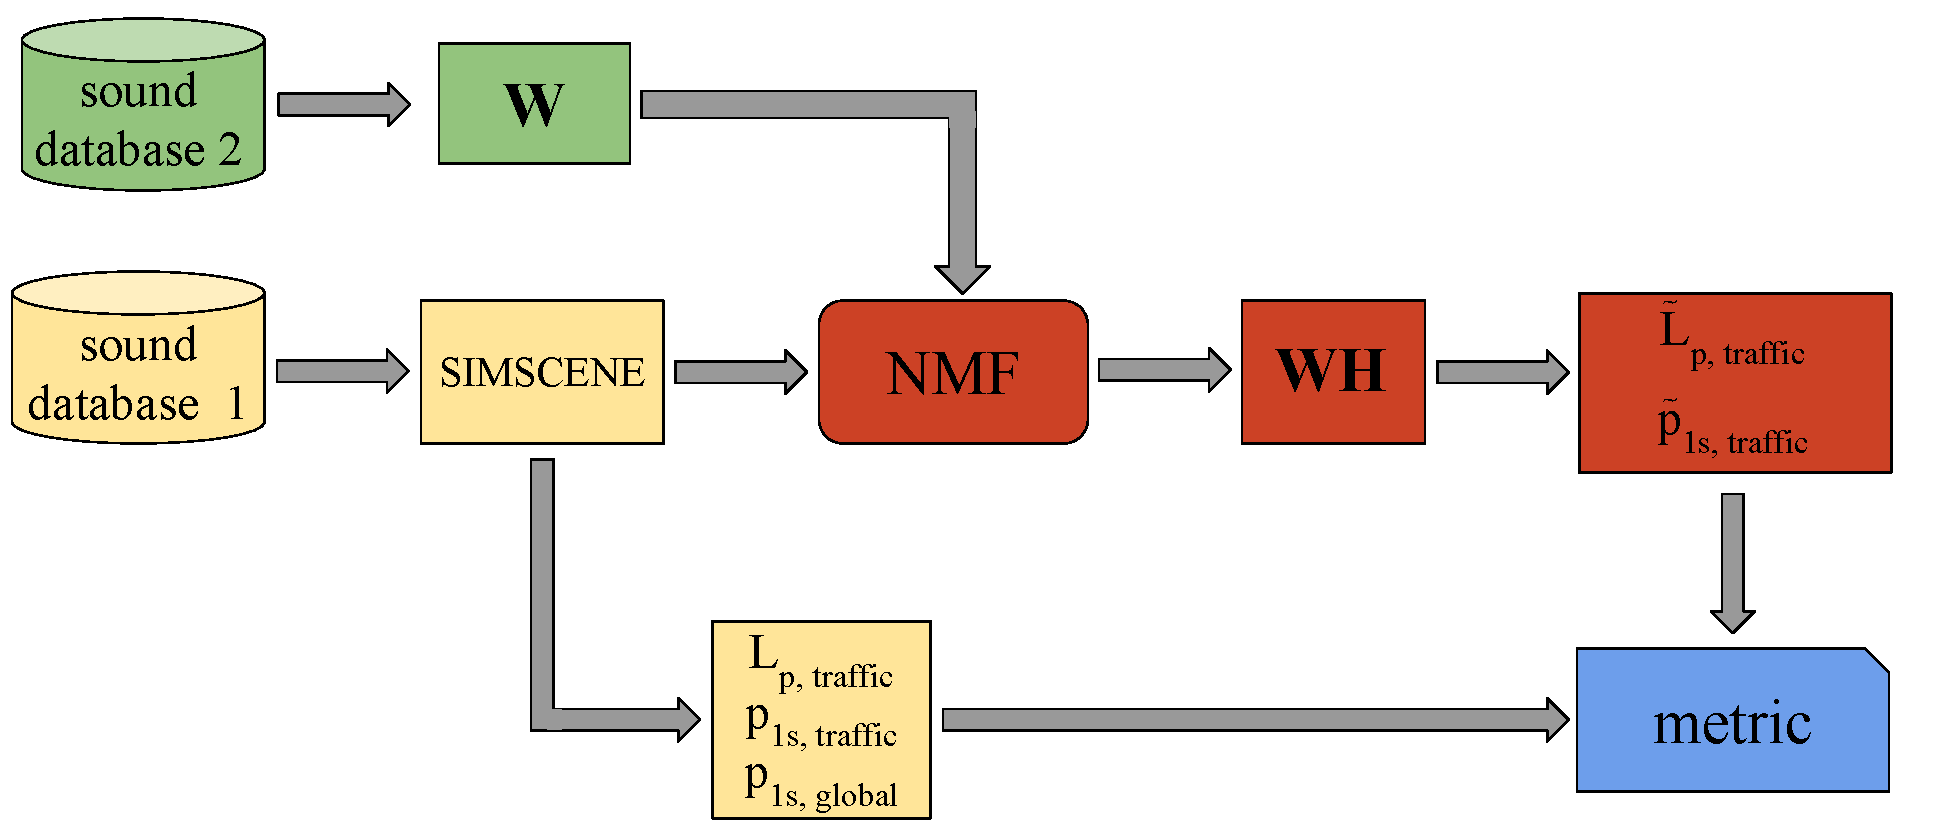
\includegraphics[width=.45\linewidth]{../image/bloc_diagram_NMF_EN.pdf}}
    \subfigure[]{\label{fig:blocDiagramFilter}	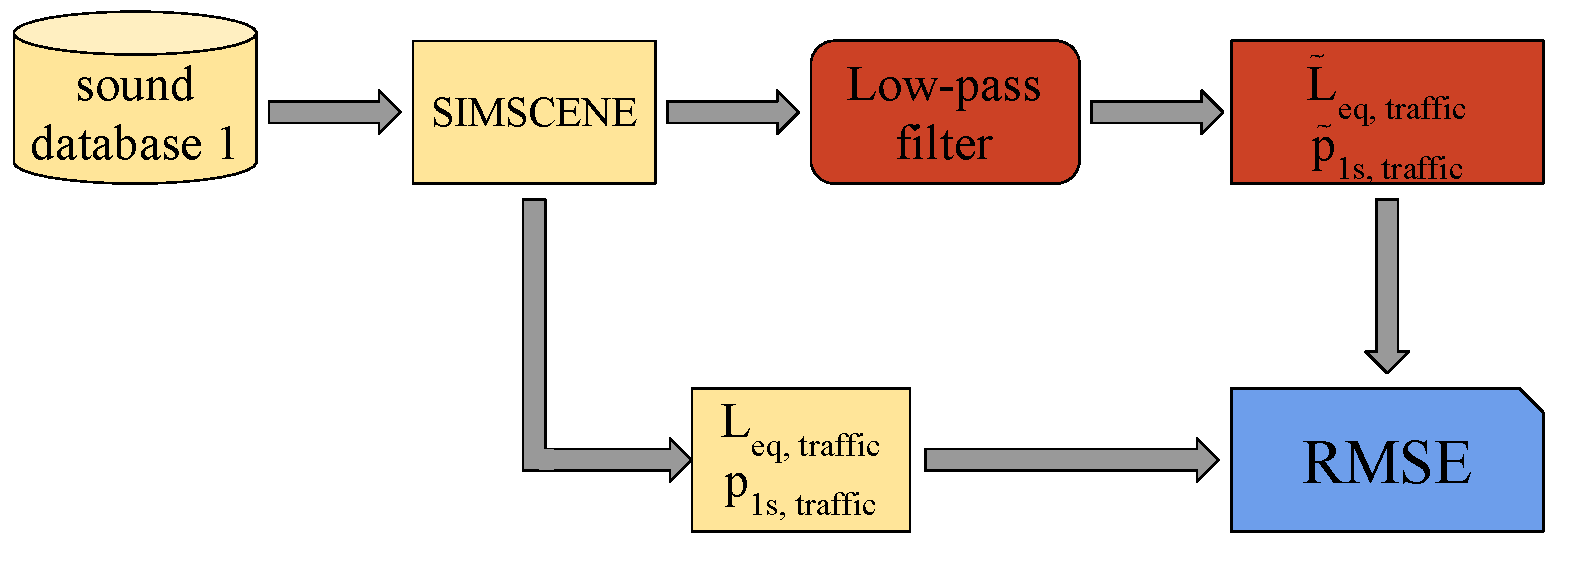
\includegraphics[width=.45\linewidth]{../image/bloc_diagram_filtrage_EN.pdf}}
    \caption{Block diagrams summed up the different step of the process for the frequency low-pass filter \ref{fig:blocDiagramFilter} and for NMF \ref{fig:blocDiagramNMF}.}
    \label{fig:blocDiagram}
\end{figure*}

Currently, sensor networks in cities are spread for multiple applications (air quality assessment, measurement of meteorological parameters, ...), including the assessment of urban noise levels. DYNAMAP project \cite{dynamap_2016} studied the establishment and feasibility of such installations. It focuses on sensor installations on specific roads at the city scale in Milan and Rome \cite{bellucci_life_2017}. In a similar way, but reduced to few neighborhoods, the CENSE project\footnote{\url{http://cense.ifsttar.fr/}} \cite{} aims to combine \textit{in situ} observations, from a sensor network, and numerical data, from noise modeling, through data assimilation techniques.

If sensors networks could improve road traffic noise estimation compared with simulated maps, the issue of the correct estimation from  measurements of the traffic sound level is still unsolved \cite{Mioduszewski}. Indeed, the urban sound environment is a complex environment gathering lots of different sounds (car passages, voices, bird's whistles, car horn \dots) that can overlap. Consequently, the traffic sound level estimation based on measurements is not trivial task.
Many recent works have focused on the detection or recognition tasks of environmental sounds without distinction between them\cite{heittola_sound_2011}, \cite{defreville_automatic_2006}, \cite{dufaux_automatic_2000}, \cite{chu_environmental_2009}. A two step process is generally followed : describe the audio files with a set of features (Spectrum Gravity Spectrum, harmonicity, Mel-Frequency Cepstral Coefficient \dots) and classify them with the help of classifiers (Support Vector Machines, Gaussian Mixture Models, Hidden Markov Model, Artifical Neural Networks). A description of there features and classifiers can be found in \cite{cowling_comparison_2003} and their application can be found in \cite{shen_environmental_2012}, \cite{beritelli_pattern_2008}, \cite{couvreur_automatic_2004}. Recently, an Anomalous Noise Events Detector has been generated in \cite{socoro_anomalous_2017} to detect the sound sources from labeled recordings that are not related to the traffic component in order not to take them into account on the estimation of the traffic sound level. If the detection of the road traffic noise is good, the detection of theses anomalous noise events stay weak and no information on the improvement on the estimation of the traffic nous level are presented.

Furthermore, this work and as well as the other works in the detection or recognition tasks, do not address the overlap of environmental sounds in an urban context. Although near major roads or ring roads traffic is predominant on all other sound sources, there are many places where road traffic overlaps with other sound sources that contribute significantly to the overall sound levels. In such case, the only detection of the traffic component does not make it possible to determine precisely its noise level. In consequence, to be effective on a wide range of sound environments, we propose in this paper to follow the blind source separation paradigm. That is, separating the contribution of the traffic from the other sources within a polyphonic scene.


One of the first and the most widely used techniques to do so is the Independent Component Analysis \cite{comon_independent_1994}. The principle is to decompose $N$ recorded signals to a sum of $P$ independent sound sources weighted by linear relations. This method is most of all suited for the 'cocktail party' issue where one tries to capture a signal among noise.  However, ICA is limited to only over determined cases ($N > P$). Furthermore, if it is suited for indoor environments where the number of sound sources is constant, it can not be fitted for an outdoor environment where the number of sources is unknown and variable and, moreover, it would be necessary to mount multiples sensors on one point to perform the source separation. A more convenient method is Non-negative Matrix Factorization (NMF) \cite{lee_learning_1999} which consists in approximating the magnitude spectrogram of an audio file from the product of two matrices. It has been widely used in the audio domain, \cite{smaragdis_non-negative_2003} \cite{wilson_speech_2008} \cite{mesaros_sound_2015}, and has already been employed for the source separation task of monaural signals of speech and music \cite{wang_musical_2005} \cite{wilson_speech_2008}. By design, this method deals with the overlaping sound sources as soon as the overlap can be resolved on the time/frequency plane. For the environmental sounds, the method has been used for the geo-localisation and classification of the sound environment, like in \cite{kumar_audio_2016} where NMF is used to classify the audio files according to the 10 cities where they have been recorded. It has also been used by Innami and Kasai in the unsupervised case \cite{satoshi_innami_nmf-based_2012} for source separation. They proposed a source separation in two steps by separating the sound background from the events first and by separating the events between them. The audio files tested results of a simulation process where a sound background (river or wind) are adding to two sound events (school chime, announcement, frog croaking, dog barging and bell ringing). If the method proposed is interesting, the main issue here is the small size of the database (only 9 sounds) on which the algorithms are tested while some sounds (frog and river) are not representative of sounds that can be found in cities.


\subsection{Proposed approach}

We propose in this paper a method based on the Non-Negative Matrix Factorization (NMF) technique to estimate the global, $\tilde{L}_{p,traffic}$, and the 1-s equivalent, $\tilde{p}_{1s,traffic}$ sound level of the traffic through the supervised and the semi-supervised approaches. To validate this approach, we consider a corpus of simulated scenes artificially created with the simulator software \textit{simScene}. The use of simulated sound scenes is necessary as it offers a full control on the design of the scenes and the knowledge of the exact contribution of the traffic component which would hardly be extracted from a recording of an urban scene ($L_{p,traffic}$ and $p_{1s,traffic}$). Both the sound scene simulation and NMF require the creation of two sound databases (figure  \ref{fig:blocDiagramNMF}). In parallel, a baseline method built from a frequency low-pass filter is computed. This method considers that road traffic is mainly composed of low frequencies and therefore can be filtered by a low-pass filter at the cut-off frequency $f_c$ (figure \ref{fig:blocDiagramFilter}). The performance of the frequency low-pass filter and NMF are then compared with the calculation of two metrics (Mean Absolute Error, normalized Root Mean Square Error). 

The remaining of the paper is organized as follows. Section \ref{part:nmf} details the technical aspect of NMF. Section \ref{part:protocol} described on the design of the environmental sound scene corpus and the experimental protocol setup. Then Section \ref{part:results} shows and discusses the results obtained during the parametric study.

%\ml{faire une figure avec un diagrame de bloc et une section proposed approach avec des sub temps/frequence nmfsup nmfsemi}

\section{Non-negative Matrix Factorization}\label{part:nmf}
\subsection{Description of NMF}
Non-negative Matrix Factorization is a matrix approximation method introduced by Lee and Seung, \cite{lee_learning_1999}, which can be used to approximate the spectrogram (obtained using a Short-Term Fourier Transform) of an audio file, $\mathbf{V}$, $\in \mathbb{R}^+_{F \times N}$ as :

\begin{equation}\label{eq:nmf}
\mathbf{V} \approx \mathbf{\tilde{V}} = \mathbf{WH}
\end{equation}

where $\mathbf{W} \in \mathbb{R}^+_{F \times K}$ is the \textit{dictionary} (or basis) matrix composed of audio spectrum and $\mathbf{H} \in \mathbb{R}^+_{K \times N}$ is the \textit{activation} matrix which summarizes the temporal evolution of each element of $\mathbf{W}$ (fig.  \ref{fig:example_NMF}).

\begin{figure}[t]
\centering
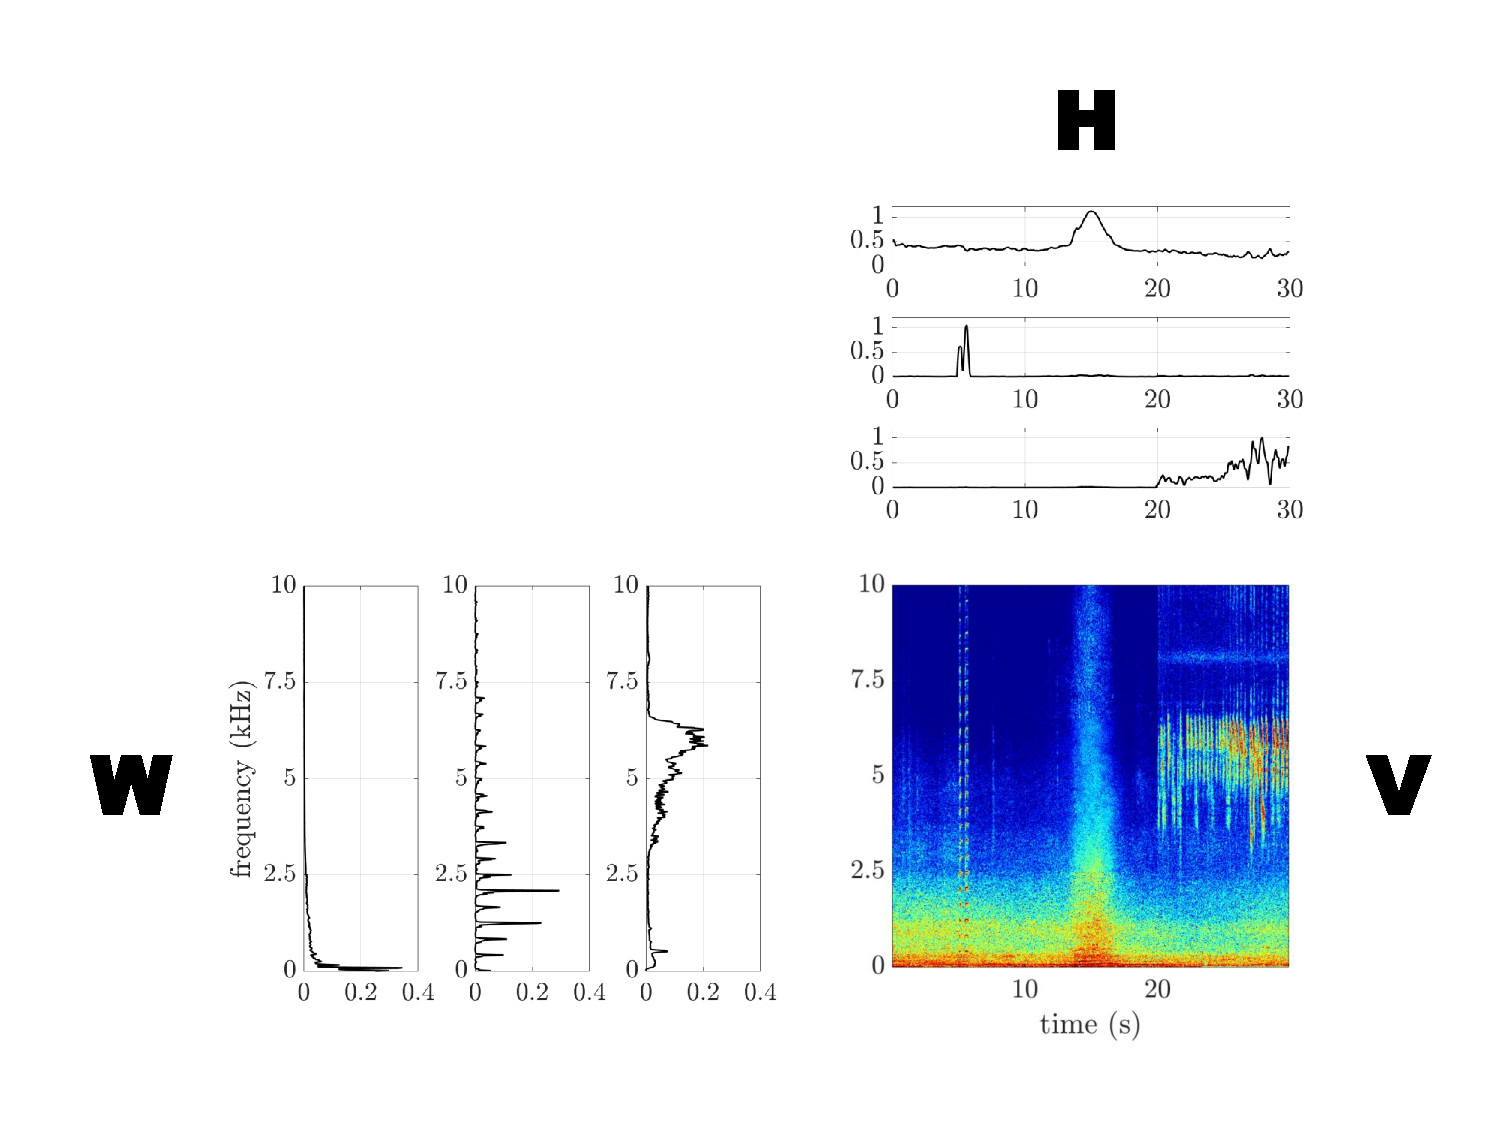
\includegraphics[width=0.9\linewidth]{../image/schema_introduction_nmf.pdf}
\caption{Example of a simple NMF  for a musical content \cite{bertin_les_2009}}
\label{fig:example_NMF}
\end{figure}

The choice of the dimensions should be such that $F\times K + K \times N < F \times N$. To estimate the quality of the approximation, an objective function is used

\begin{equation}\label{eq:min-D-WH}
\underset{\mathbf{H} \geq 0, \mathbf{W} \geq 0}{\min} D\left(\mathbf{V} \vert \vert \mathbf{\tilde{V}}\right).
\end{equation}

The operator $D(x\vert y)$ is a divergence calculation such as:
\begin{equation}
D\left(\textbf{V} \vert\vert \mathbf{\tilde{V}} \right) = \sum_{f = 1}^{F} \sum_{n = 1}^{N} d_{\beta}
\left(\textbf{V}_{fn} \vert \left[ \textbf{WH} \right]_{fn} \right)
\end{equation}

and usually belongs to the $\beta-$divergence class \cite{fevotte_nonnegative_2009} in which the well known Euclidean distance (eq. \ref{eq:def_distEUC}) and the Kullback-Leibler divergence (eq. \ref{eq:def_divKL}) belong

\begin{subequations}\label{eq:divBetaGenerale}
\begin{numcases}{d_{\beta}(x\vert y) =}
    \frac{1}{2}(x-y)^2, & $\beta = 2$, \label{eq:def_distEUC}\\
    x\log \dfrac{x}{y} - x + y, & $\beta = 1$.\label{eq:def_divKL}
\end{numcases}
\end{subequations}

Prior knowledge on the content can be adjusted with the addition of constraints (like the smoothness or the sparsness criteria \cite{virtanen_monaural_2007}) in the objective function (equation (\ref{eq:min-D-WH})) to better take account prior knowledge of the sources.

Algorithms have been proposed to solve the minimization problem (\ref{eq:min-D-WH}) iteratively such as the multiplicative update \cite{lee_algorithms_2000}, the alternating least square method \cite{cichocki_regularized_2007}, the projected gradient \cite{lin_projected_2007} \dots Here, the multiplicative update is chosen as it ensure non-negative results of which convergence has been proved \cite{fevotte_algorithms_2011}.

\subsection{Supervised NMF}
First, supervised NMF is used: the \textit{dictionary} includes audio spectrum of urban sound sources as, in the urban environments, a lot of different sound sources present are known and their spectrum can be obtained. The \textit{basis} are then the unknown to estimate. In the first iteration, $\mathbf{H}$ is initialized randomly, then it is updated by the generic algorithm

\begin{equation}\label{eq:updateH_Sup}
\textbf{H}^{(i+1)} \leftarrow \textbf{H}^{(i)}.\left(\frac{\textbf{W}^T \left[\left(\textbf{WH}^{(i)} \right)^{(\beta-2)}.\textbf{V} \right]}{\textbf{W}^T \left[\textbf{WH}^{(i)} \right]^{(\beta-1)}}\right)^{\gamma(\beta)}
\end{equation}

with $\gamma(\beta) = \frac{1}{2-\beta},$ for $\beta < 1$, $ \gamma(\beta) = 1$, for $\beta \in \left[1,2\right]$ and $\gamma(\beta) = \frac{1}{\beta-1}$ for $\beta > 2$. The product $A.B$ and $A/B$ symbolized the Hadamard product and ratio. As in the supervised approach, the position in $\mathbf{W}$ of traffic component is known, the source separation of this sound source is made by extracting the dictionary and basis elements related, 

\begin{equation}\label{eq:separationExtraction}
\mathbf{\tilde{V}}_{traffic} = \left[ \mathbf{WH} \right]_{traffic}.
\end{equation}

%or by generating a soft mask, $\mathbf{M_s}$,
%
%\begin{equation} \label{eq:definitionMask}
%\mathbf{M_s} = \frac{\left[\mathbf{W} \mathbf{H}\right]_{traffic}}{\mathbf{W H}},
%\end{equation}
%
%which allows to determine the spectrogram of the traffic component, $ \mathbf{\tilde{V}}_{traffic}$
%
%\begin{equation}\label{eq:separation}
%\mathbf{\tilde{V}}_{traffic} = \mathbf{M_s}.\mathbf{V}.
%\end{equation}

\subsection{Semi-supervised NMF}

One of the main issue with the supervised approach is 

To better take account for the diverse nature of urban scenes, semi-supervised NMF can be useful as it has been proposed \cite{lee_semi-supervised_2010} to offer more flexibility. This method consists in composing the \textit{dictionary} with a fixed part $\mathbf{W_s} \in \mathbb{R}^+_{F\times K}$, composed in our case of spectrum representative of road traffic and with a mobile part, $\mathbf{W_r} \in \mathbb{R}^+_{F\times J}$ with $J <<K$, that is updated. Here, $J = 2$. The aim is to include in $\mathbf{W_r}$ the element that are not related with the traffic. The problem (\ref{eq:nmf}) become

\begin{equation}
\mathbf{V} \approx \mathbf{W_s H_s}+ \mathbf{W_r H_r}.
\end{equation}

In a similar way as to solve the equation \ref{eq:min-D-WH}, $\mathbf{W_r}$, $\mathbf{H_r}$ and $\mathbf{H_s}$ are successively updated with the relations (\ref{eq:WH-SSupdate}):

{\scriptsize
\begin{subequations}\label{eq:WH-SSupdate}
\begin{align}
\mathbf{W_r}^{(i+1)} &\leftarrow \mathbf{W_r}^{(i)}.\left(\frac{\left[\left(\mathbf{W_r H_r}^{(i)} \right)^{(\beta-2)}.\mathbf{V} \right]\mathbf{H_r}^T}{\left(\mathbf{W_r H_r}^{(i)} \right)^{(\beta-1)}\mathbf{H_r}^T}\right)^{\gamma(\beta)}, \label{eq:W_r_SS}\\
\mathbf{H_r}^{(i+1)} &\leftarrow \mathbf{H_r}^{(i)}.\left(\frac{\mathbf{W_r}^T \left[\left(\mathbf{W_r H_r}^{(i)} \right)^{(\beta-2)}.\mathbf{V} \right]}{\mathbf{W_r}^T \left(\mathbf{W_r H_r}^{(i)} \right)^{(\beta-1)}}\right)^{\gamma(\beta)}, \label{eq:H_r_SS}\\
\mathbf{H_s}^{(i+1)} &\leftarrow \mathbf{H_s}^{(i)}.\left(\frac{\mathbf{W_s}^T \left[\left(\mathbf{W_s H_s}^{(i)} \right)^{(\beta-2)}.\mathbf{V} \right]}{\mathbf{W_s}^T \left(\mathbf{W_s H_s}^{(i)} \right)^{(\beta-1)}}\right)^{\gamma(\beta)}.\label{eq:H_s_SS}
\end{align}
\end{subequations}}

%This approach has been used TO COMPLETE.

\subsection{Thresholded constrained NMF}

A last approach is tested based on unsupervised NMF. Usually, $\mathbf{W}$ is learnt with the help of a learning corpus by initiated it randomly. Here, as the concerned sound source is known and audio samples of car passages are available, a initial dictionary, $\mathbf{W_0}$, is learnt by converting the audio files in the spectra domain . Then NMF is performed where $\mathbf{W}$ (eq. \ref{eq:updateW_unsup}) and $\mathbf{H}$ (eq.  \ref{eq:updateH_Sup}) are updated iteratively. 

\begin{equation}\label{eq:updateW_unsup}
\textbf{W}^{(i+1)} \leftarrow \mathbf{W}^{(i)}.\left(\frac{\left[\left(\mathbf{W}^{(i)}\mathbf{H} \right)^{(\beta-2)}.\mathbf{V} \right]\mathbf{H}^T}{\left[\mathbf{W}^{(i)}\mathbf{H} \right]^{(\beta-1)}\mathbf{H}^T}\right)^{\gamma(\beta)}
\end{equation}

After $N$ iterations, a measure of similarity $D_{\theta}\left(\mathbf{W_0} \vert \vert \mathbf{W} \right)$ between $\mathbf{W_0}$ and the get dictionary $\mathbf{W}$ for each element $k$ is computed through a cosine similarity, 

\begin{equation}
\cos \theta = \frac{\mathbf{W}.\mathbf{W_0}}{\vert \vert \mathbf{W}  \vert \vert . \vert \vert \mathbf{W_0} \vert \vert}.
\end{equation}

$\cos \theta = 1$ means that the elements are identical (the $k$-th element of $\mathbf{W}$ is then considered as traffic element) whereas $\cos \theta = 0$ means that the elements are diametrically opposed. This measure allows a normalized and an invariant scale estimation of the similarity. It is then sort in descending order. The elements in $\mathbf{W}$ that can belong to $\mathbf{W}_{traffic}$ are then selected by a \textit{hard thresholding} method (Figure \ref{fig:W_THC_NMF}). It is defined as :

\begin{equation}
\mathbf{W}_k \in \mathbf{W}_{k,traffic} \quad \text{iff} \quad D\left(\mathbf{W}_{0,k} \vert \vert \mathbf{W}_{k} \right) > t
\end{equation}

\begin{figure}[hbtp]
\centering
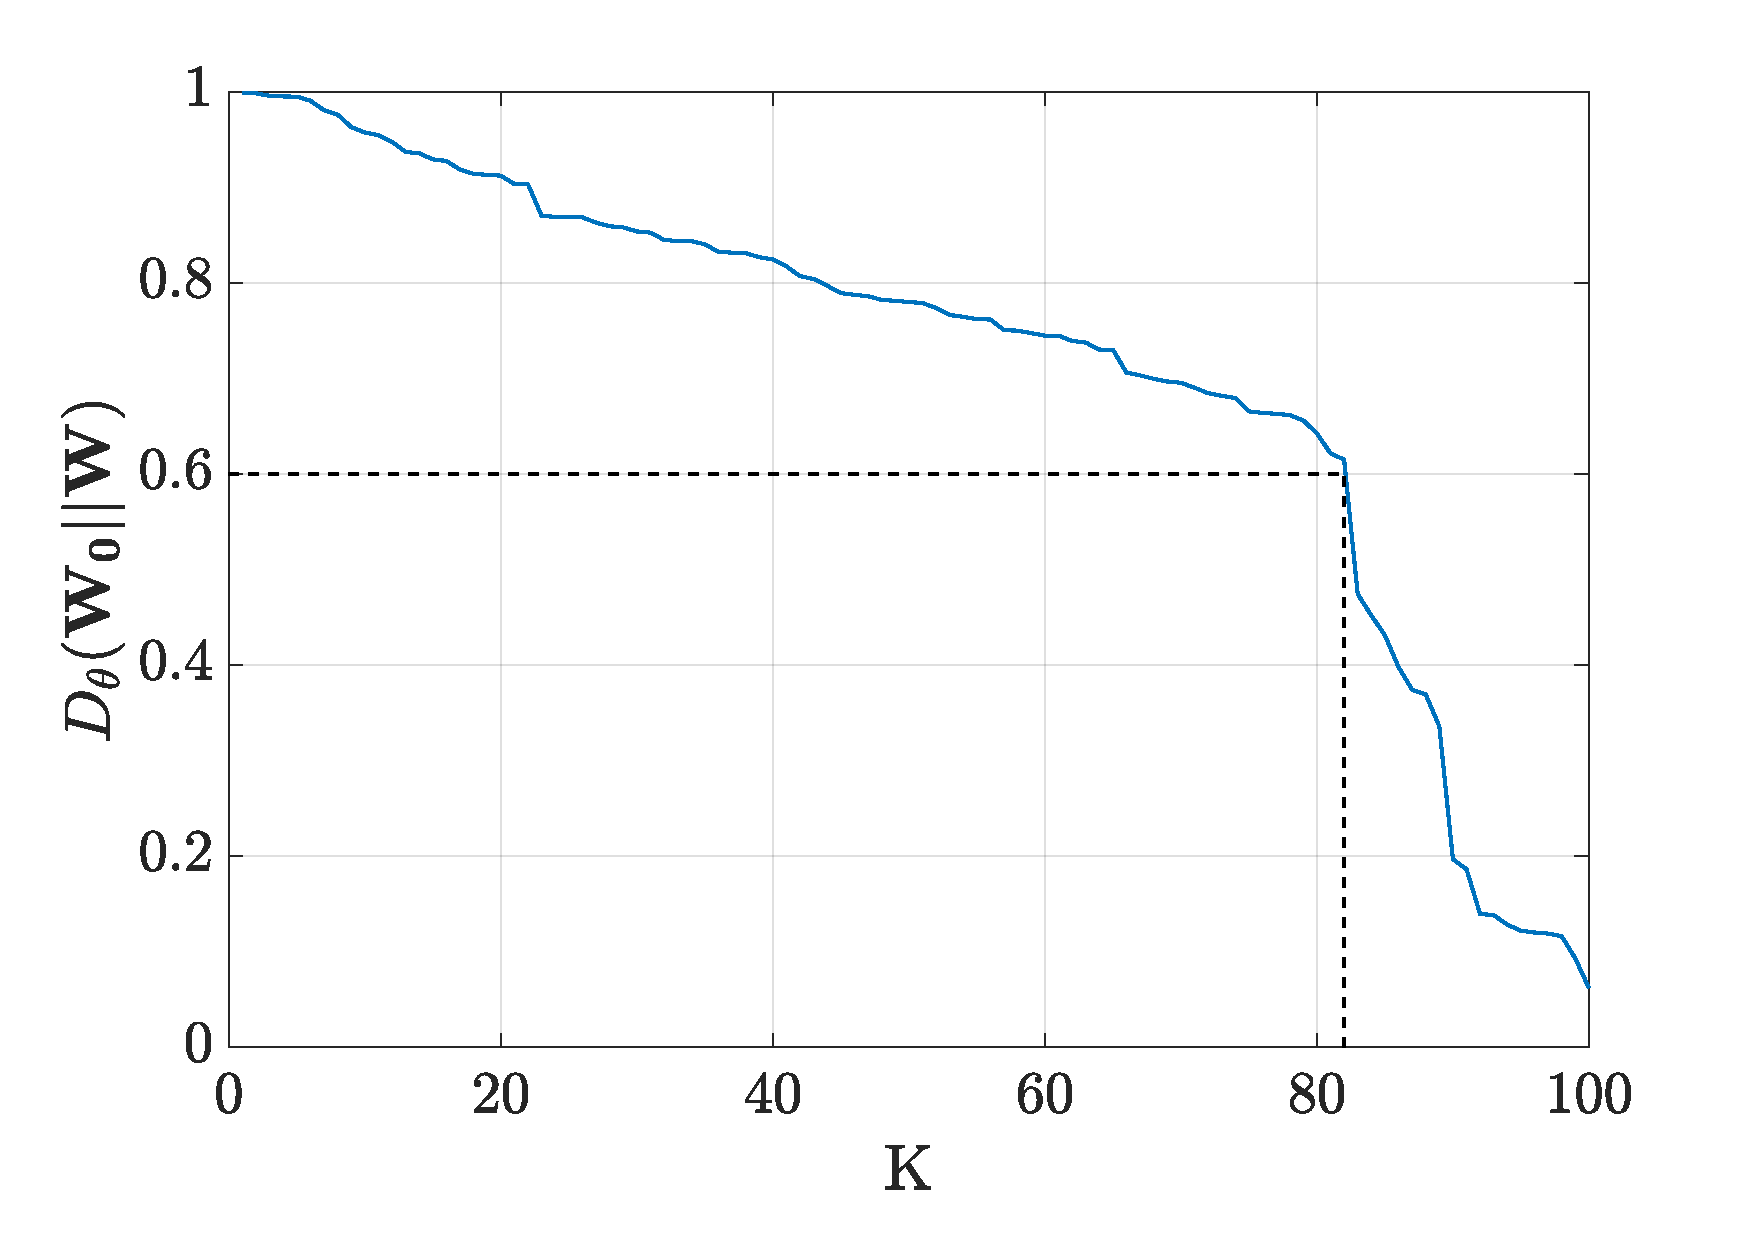
\includegraphics[width=0.8\linewidth]{../image/distanceCosLinDisplay.pdf}
\caption{Example of the $\mathbf{W}_{traffic}$ extraction from the sorted cosine similarity with a threshold $t = 0.6$. The $82$-nd first elements are considered as traffic component.}
\label{fig:W_THC_NMF}
\end{figure}

Other thresholding methods as the \textit{soft} and the \textit{firm} and multiples way to display the distance through a sigmoïd or a Radial Basis Function have been investigated. A fast parametric study has revealed that the \textit{hard} tresholding method  with a linear representation of the similarity according to $K$ (see fig. \ref{fig:W_THC_NMF}) was the best way to get better performances. 


\section{Experimental protocol}\label{part:protocol}

In order to validate the usefulness of considering NMF framework to estimate the road traffic noise level, one need to have a reference level. It can hardly be measured or even annotated from real life recordings. Thus,  simulated sound scenes are used to assess the performance of the proposed NMF. This offers a controlled framework to design specific sound environments in which all the traffic component is known. Then, the road traffic sound levels estimated with the method can be compared to the real ones, introduced within each simulated sound scene.

\subsection{Environmental sound scene corpus}

A corpus is designed with the \textit{simScene} software\footnote{Open-source project available at: \url{https://bitbucket.org/mlagrange/simscene}}. \textit{simScene} \cite{rossignol_simscene:_2015} is a simulator that creates sound scenes in a .wav format by summing audio samples that come from an isolated sound database. 

This database is divided in two categories: $i)$ the \textit{event} category which are the brief sounds (from 1 to 20 seconds) that are considered as salient including 245 sound event samples divided in 19 sound classes (\textit{ringing bell, birds, sweeping broom, car horn, car passages, hammer, drill, coughing, barking dog, rolling suitcase, closing door, plane, siren, footstep, storm, street noise, train, tramway, truck and voice}) and $ii)$ the \textit{background} category that includes all the sounds that are of long duration and whose acoustic properties do not vary with respect to time. 154 sound samples belong to this category divided in 9 sound classes (\textit{birds, construction site noise, crowd, park, rain, children playing in schoolyard, constant traffic noise, ventilation, wind}). The sound class \textit{car passages} comes from 60 recordings of 2 cars made on the Ifsttar's runway on different speeds with multiple gear ratio. The other audio files have been found online (\textit{freesound.org}) and within the \textit{UrbanSound8k} database \cite{salamon_dataset_nodate}. Each sound classes are composed of multiples samples (\textit{bird01.wav}, \textit{bird02.wav} \dots). 
The software allows the user to control some parameters (number of events of each class that appear in the mixture, elapsed time between each sample of a same class, presence of a fade in and a fade out \dots) completed with a standard deviation that may brings some random behavior between the scenes. Furthermore, an audio file of each sound class present in the scene can be generated that allows to know its exact contribution as well as a text file that summarizes the time presence of all the events.\\

\begin{figure}[t]
\centering
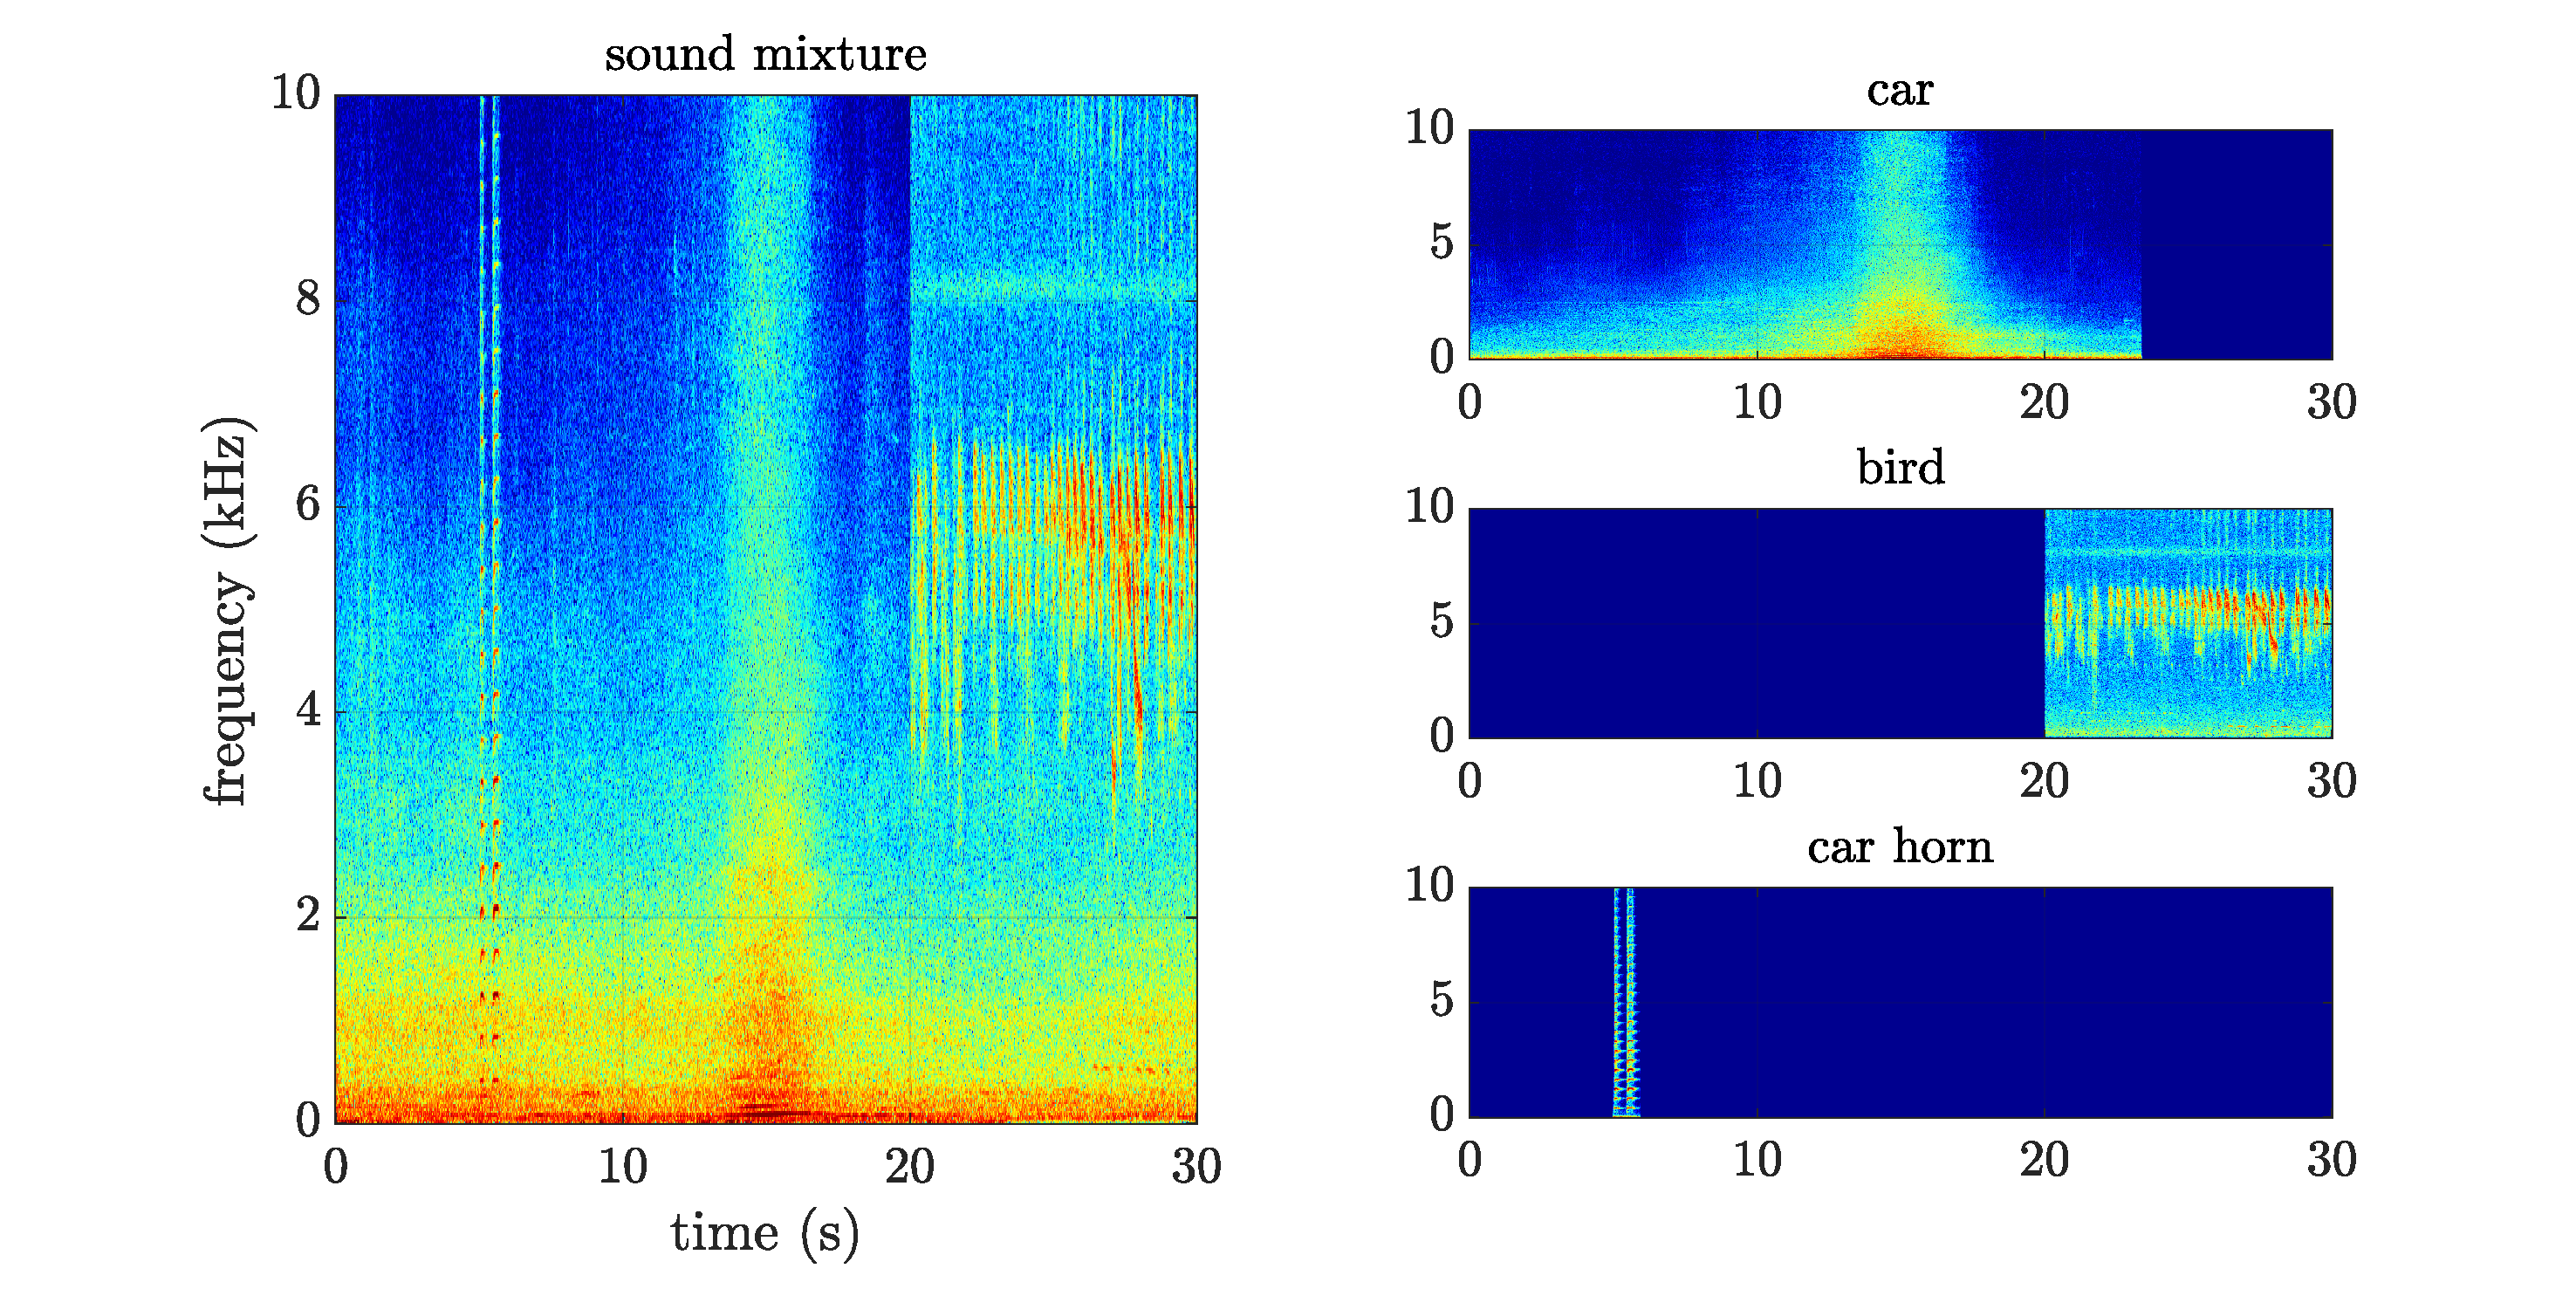
\includegraphics[width=\linewidth]{../image/exampleSimScene2.pdf}
\label{fig:exampleSimScene}
\caption{Example of a sound scene composed of 3 sound classes (car, bird, car horn)}
\end{figure}

This database enables creating realistic urban sound scenes from the road traffic point of view \cite{gloaguen_creation_2017}. A sound mixing corpus is composed of 6 sub-corpus of 25 audio files each lasting 30 seconds. Each sub-corpus is characterized by a specific generic sound class that summed with traffic will make the estimation of the traffic level more difficult. The classes are : \textit{alert} (car horn, siren), \textit{animals} (barking dog , whistling birds), \textit{climate} (wind, rain), \textit{humans} (crowd noise and voice), \textit{mechanics} (different metallic and construction site noises) and \textit{transportation} (train, tramway and plane). In each file, traffic component is present as the sum of the background and event traffic sounds and is mixed with the sound classes. The sound classes that are not related to the traffic component are summed up as the \textit{interfering} sound class. To test different scenarios, each audio file is duplicated with the traffic sound level of the entire sound scene, $L_{p,traffic}$, fixed to a specific level according to the sound level of the \textit{interfering} class, $L_{p,interfering}$ following the relation (\ref{eq:tir}).

\begin{equation}\label{eq:tir}
TIR = L_{p,traffic}-L_{p,interfering}
\end{equation}

with the \textit{Traffic Interference Ratio} $TIR = \left[-12, -6, 0, 6, 12\right]$. When $TIR = -12$, the traffic component is then less present than when $TIR = 12$ where it is predominant on the \textit{interfering} class. The 1 second equivalent sound pressure level, $p_{1s,traffic}$, is also calculated (figure \ref{fig:exampleScene}). Finally, the number of scenes designed is 750 (6 sub-corpus $\times$ 25 scenes $\times$  5 TPR values).

\begin{figure*}
\centering
   \begin{minipage}[c]{.32\linewidth}
      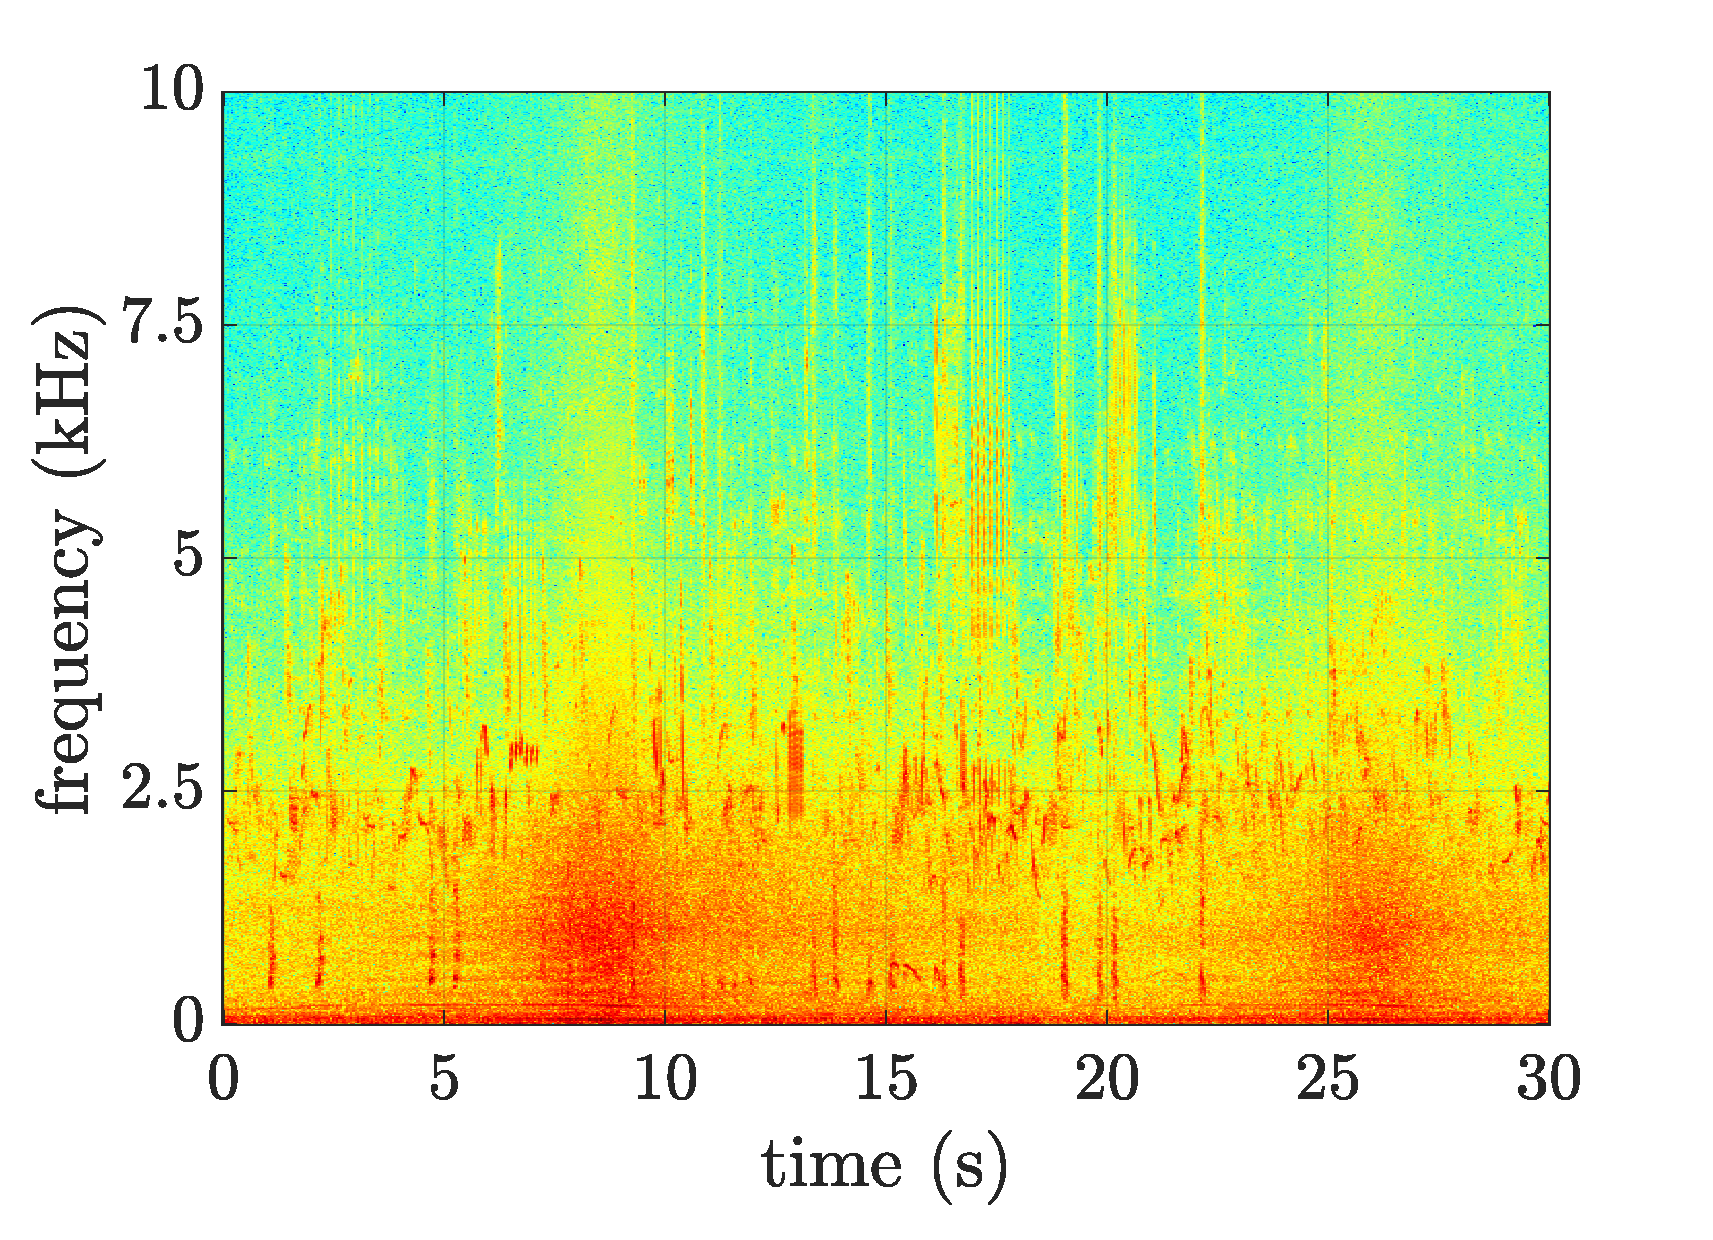
\includegraphics[width =\linewidth]{../image/spectrogramExample.pdf}
   \end{minipage}
   \begin{minipage}[c]{.32\linewidth}
      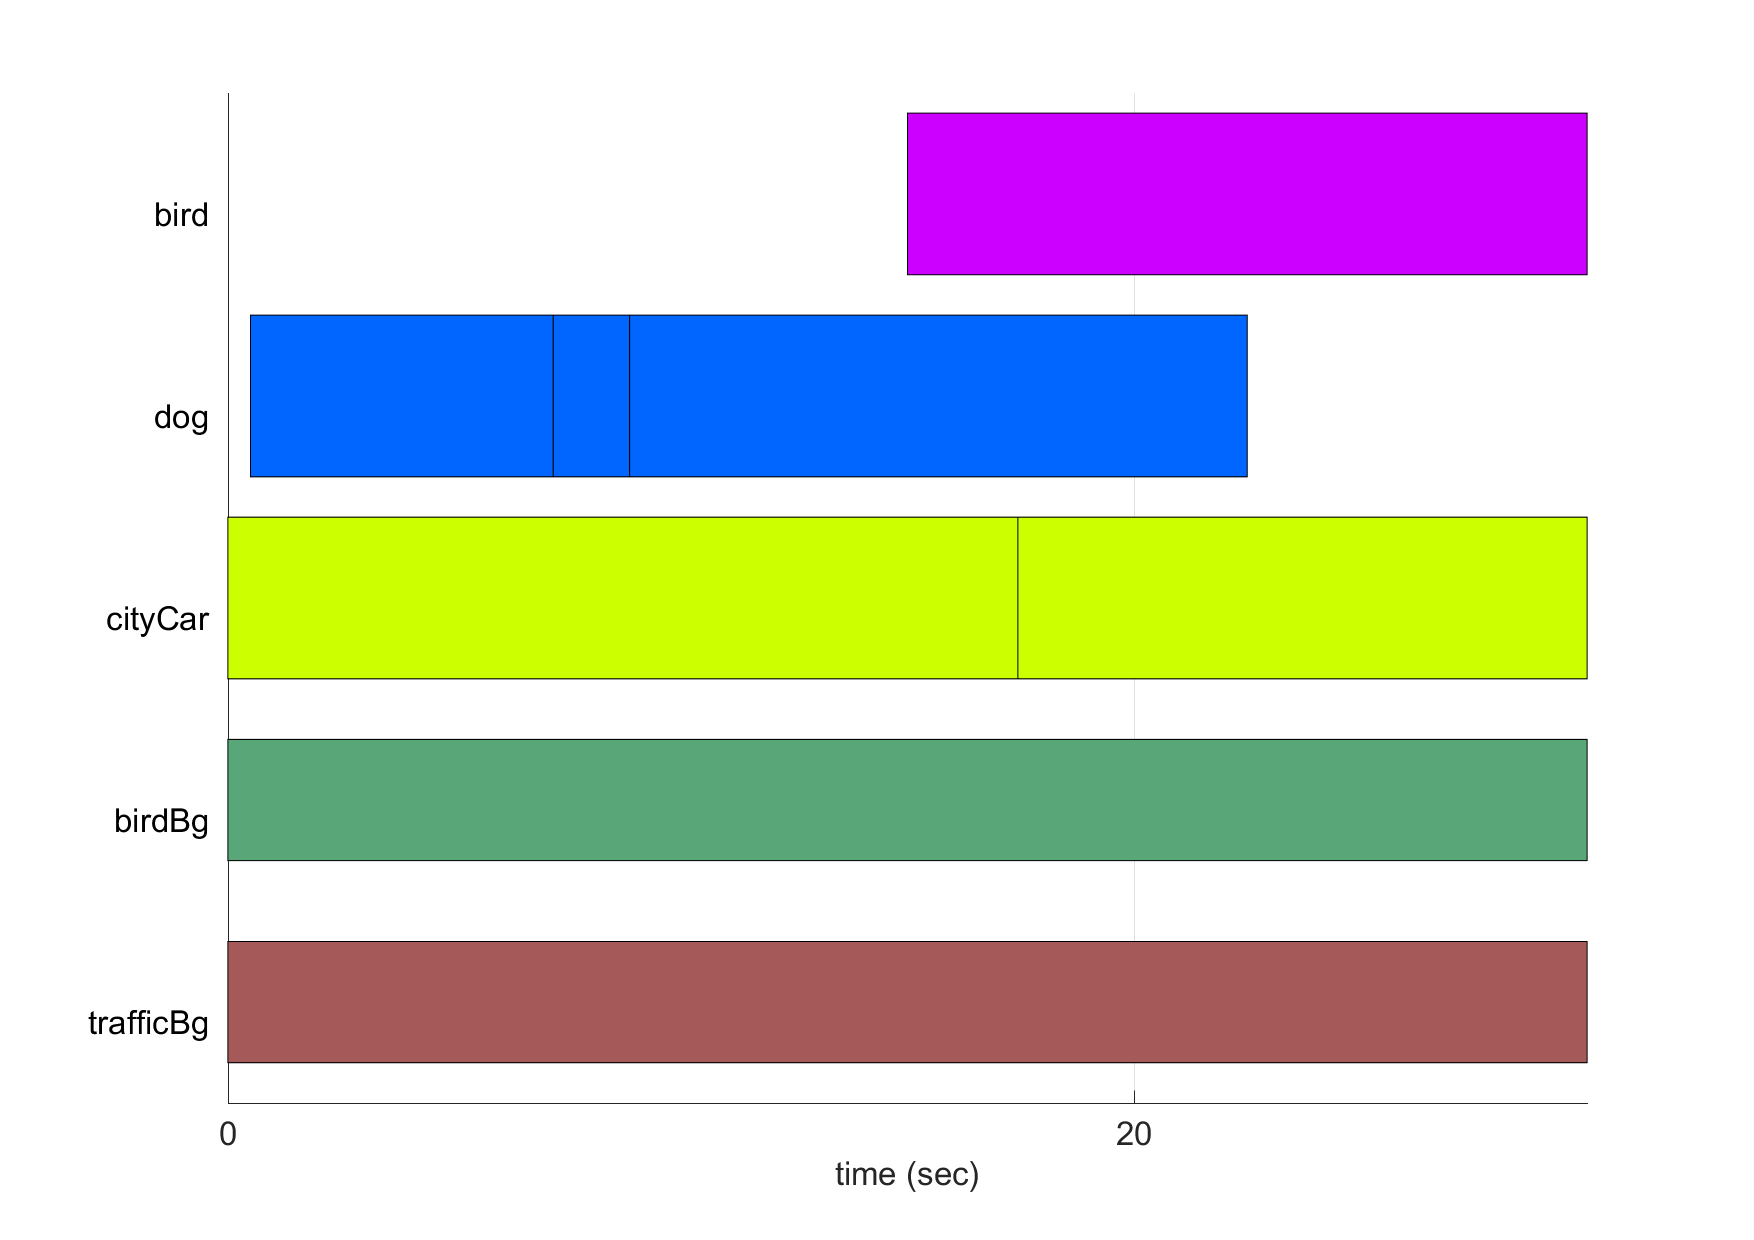
\includegraphics[width =\linewidth]{../image/animals_10-pianoRoll.png}
   \end{minipage}
   \begin{minipage}[c]{.32\linewidth}
      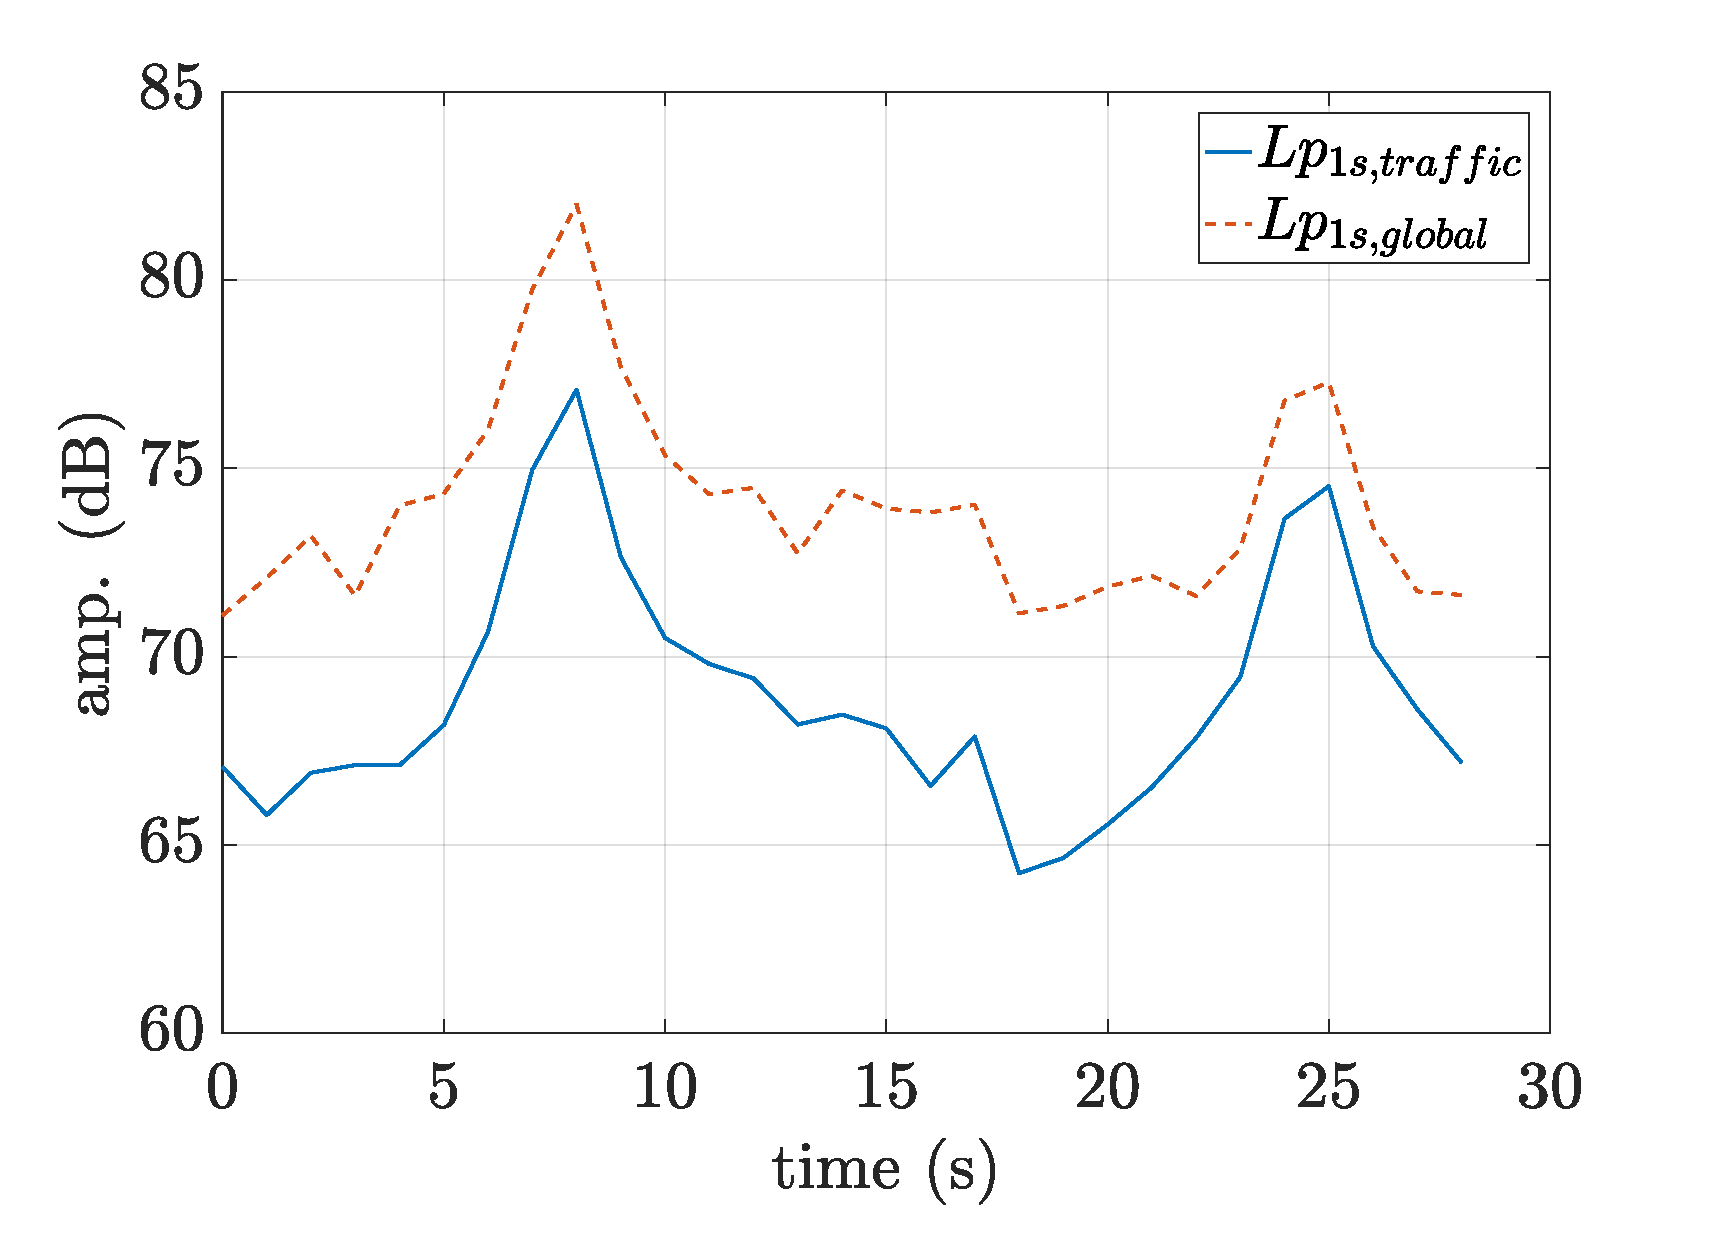
\includegraphics[width =\linewidth]{../image/evolutionLpExample.pdf}

   \end{minipage}
\caption{Example of a scene of the \textit{animals} sub corpus. Spectrogram (on left), \textit{Piano Roll} of the different sound classes (on the middle) and 1-s equivalent sound level of the traffic, $Lp_{1s,traffic}$ and of the global sound scene, $Lp_{1s,global}$(on right)}
\label{fig:exampleScene}
\end{figure*}

\subsection{Experiment}

The experiment consists in estimating the traffic road sound level of the 6 environmental sound sub-corpus (\textit{alert} (al), \textit{animals} (an), \textit{humans} (hu), \textit{climate} (cl), \textit{mechanics} (me), \textit{transportation} (tr)) and for 5 $TIR$ ([-12 -6 0 6 12] dB). First, the spectrogram $\mathbf{V}$ of each sound scene is built with a window size $w = 2^{12}$ with a 50 $\%$ overlap and a number of point $nfft = 2^{12}$. Therefore, the dimensions of $V$ are $F$ = 2049 and $N$ = 664. 

The first estimator to determine the traffic sound level is the basic frequency low-pass filter which depend only on the cut-off frequencies $f_c$ = [500 1k 2k 5k 10k 20k] Hz. The spectrograms $\mathbf{V}$ are filtered and the remaining energy is then considered as traffic component (eq. \ref{eq:v_tr_filtered}). 

\begin{equation}\label{eq:v_tr_filtered}
\mathbf{\tilde{V}}_{traffic} = \mathbf{V}_{f_c}.
\end{equation}

The second estimator is NMF. Multiples parameters are involved here between the building of the dictionary and the performed NMF. 

\subsubsection{Dictionary building}

The dictionary is built from a second sound database dedicated specifically to this task. It is composed of 53 audio files of passing cars. These records have been made on the Ifsttar's runway with the same conditions that the records made for the \textit{simScene} database but with two different cars (). First, for each audio file, its spectrogram is calculated with fixed parameters ($w$, 50 $\%$ overlap, $nfft$). Then time/frequency windows with $w_t \times F$ dimension are applied without overlapping on the spectrogram in order to consider several spectrum for each audio file. $w_t$ is fixed at $wt = [0.5 1]$ second. In each window, the root mean square value is calculated on each frequency bin to reduce the different spectrum in one spectra. Since the number of elements given by processing all the sound database is high, in order to reduce the computational and delete redundant information, a $K$-means clustering is applied to reduce the number of spectrum to $K = \left[ 25, 50, 100 \right]$. A special case is added where the root mean square of \textit{all} the spectrogram is applied. Each audio file generates one element $k$ of $\mathbf{W}$. An example that illustrates the process can be found on figure \ref{fig:dictionaryExtraction} on 3 seconds extract of a spectrogram of a car passage (fig. \ref{fig:specW}). In the case where $w_t$ = 1 second , 3 elements are therefore extracted of the spectrogram while in the case where $w_t$ = \textit{all}, all the spectrogram is reduced to one element (fig. \ref{fig:ElementW}).

\begin{figure}
    \centering
\begin{minipage}[t]{\linewidth}
    \subfigure[]{\label{fig:specW}
    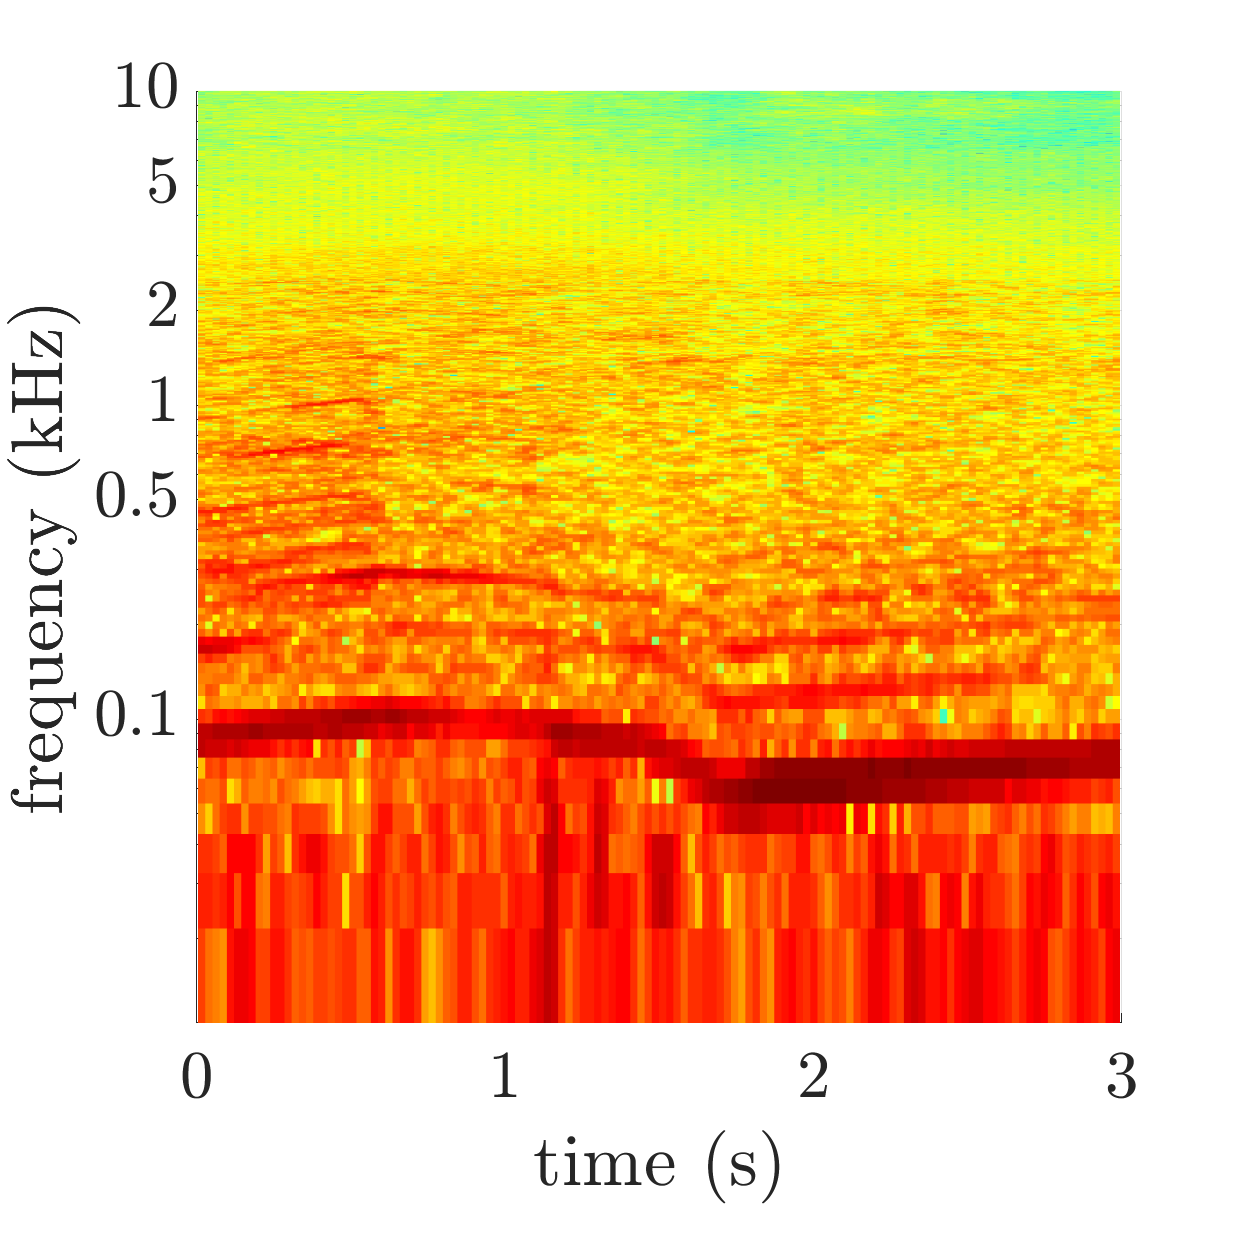
\includegraphics[width=.45\linewidth]{../image/extractionDictionary3Example.pdf}}
    \subfigure[]{\label{fig:ElementW}
    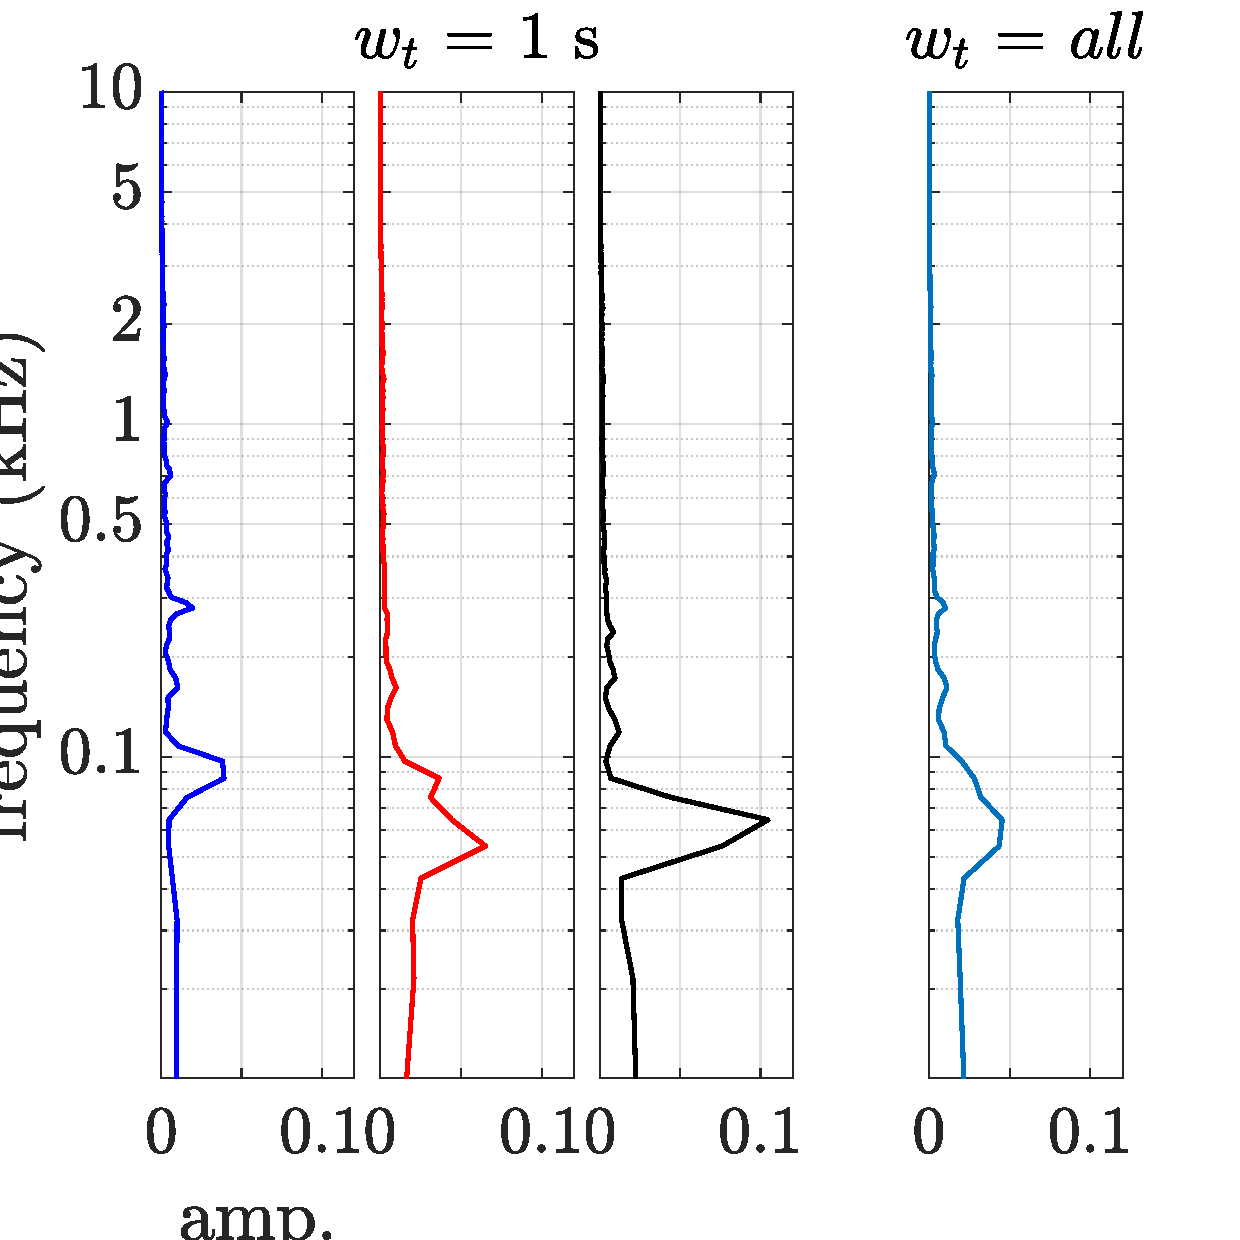
\includegraphics[width=.45\linewidth]{../image/extractionDictionary4Example.pdf}}
    
    \caption{Example of the creation of the dictionary from the spectrogram of a three seconds sample of car passage with two temporal windows ($w_t$ = 1 and $w_t = all$) expressed in a logarithmic scale.}
    \label{fig:dictionaryExtraction}
    \end{minipage}
\end{figure}

Each $k$ element of $\mathbf{W}$ is normalized such as $\vert \vert \mathbf{W_k} \vert \vert = 1$ with $\vert \vert \bullet \vert\vert$ the $\ell$-1 norm.\\
Table \ref{tab:dictionary_factors} summarizes the parameters and their related values.

\begin{table}[h]
\centering
\begin{tabular}{cccc}
Parameter &  \multicolumn{3}{c}{value}\\ \hline
$K$ & 25  & 50 & 100 \\ \hline
$\mathbf{w_t}$ (s)& 0.5 & 1  & \textit{all}
\end{tabular}
\caption{Summary of the dictionary parameters}
\label{tab:dictionary_factors}
\end{table} 

\subsubsection{Performed NMF}

Supervised and semi-supervised NMF are performed for 400 iterations which is sufficiently enough to get a stabilized reconstruction. THC-NMF is performed on a lower number of iteration (60) to prevent $\mathbf{W}$ to not deviate to much from the initial dictionary. The spectrogram $\mathbf{V}$ and the dictionary $\mathbf{W}$ are expressed on two different formats: with a linear frequency scale ($\Delta f \approx 10.8$ Hz) and with third octave bands (29 bands). Theses two methods are considered to compare a fine grain approach (the linear scale) with a coarser one (the third octave bands) as it reduces the number of frequency bins and allows to reduces the number of bands in the high frequencies where the traffic component is less present.  Furthermore, in the case of the linear frequency scale and for supervised and semi-supervised NMF, $\mathbf{V}$ and $\mathbf{W}$ are filtered at the frequencies $f_c$ in order to focused the reconstruction of the signal of the low frequency bins. Nevertheless, if NMF is performed with filtered elements ($\mathbf{V}_{f_c}$ and $\mathbf{W}_{f_c}$) to determine $\mathbf{H}_{f_c}$, the traffic signal reconstruction is done with the original dictionary $\mathbf{W}$, as

\begin{equation}
\mathbf{\tilde{V}}_{traffic} = \left[\mathbf{WH}_{f_c}\right]_{traffic}.
\end{equation}

With the third octave frequency scale, only the case $f_c = 20$ kHz is applied. Finally, for the THC NMF, the threshold is define between 0.20 and 0.70 with a 0.01 step. Table \ref{tab:estimation_factors} summarizes the parameters and the related values.

\begin{table*}[]
\centering
\begin{tabular}{lcccccc}
Parameter &  \multicolumn{6}{c}{value}\\ \hline
$\mathbf{TIR}$ (dB) & -12 & -6 & 0 & 6 & 12 &  \\ \hline
\textbf{sub-classes} & alert & animals & climate & humans & transportation & mechanics \\ \hline
\begin{tabular}[l]{@{}c@{}}\textbf{spectral} \\ \textbf{representation}\end{tabular} & \multicolumn{3}{c}{linear} & \multicolumn{3}{c}{third octave}\\ \hline
$\mathbf{\beta}$ & \multicolumn{3}{c}{1} & \multicolumn{3}{c}{2} \\ \hline
$\mathbf{f_c}$ (kHz) & 0.5 & 1 & 2 & 5 & 10 & 20 \\ \hline
\textbf{method} & \multicolumn{2}{c}{filter} & supervised NMF & semi-supervised NMF & THC NMF \\ \hline
$\mathbf{t}$ & \multicolumn{6}{c}{0.20:0.01:0.70} \\ \hline
\end{tabular}
\caption{Summary of the different parameters taken into account in the frequency low-pass filter and NMF process and their values for the estimation of the traffic sound level}
\label{tab:estimation_factors}
\end{table*}


\subsubsection{Metrics}
The performances of the two estimators of the road traffic sound level are assessed through the calculation of two metrics.

\begin{itemize}

\item The Mean Absolute Error, $MAE$, expresses the quality of the long-term reconstruction of the signal. It consists in the average over the $N$ sound scenes of the absolute difference between the exact and estimated traffic sound level in dB,

\begin{equation}
MAE = \frac{\sum_{n = 1}^N\vert L^n_{p,traffic}-\tilde{L}^n_{p,traffic} \vert}{N}.
\end{equation}

\item The normalized short-term Root Mean Square Error, $nRMSE$, calculates, for each sound scene, the error between the exact and estimated road traffic 1-s equivalent sound level of each file normalized by the 1-s equivalent sound level of the global scene, $p^t_{1s,global}$, in the linear scale,

\begin{equation}
nRMSE = \sqrt{\frac{1}{T}\sum_{t = 1}^T \left(\frac{p^t_{1s,traffic}-\tilde{p}^t_{1s,traffic}}{p^t_{1s,global}}\right)^2}
\end{equation}

where $T$ is the number of temporal bin in the signal. The linear scale is here more relevant as it is more sensitive to the error on the high sound levels than the dB scale. Then for one combination of factors, the $N$ $nRMSE$ calculated are averaged.\\
\end{itemize}

In all, according the table \ref{tab:dictionary_factors} and \ref{tab:estimation_factors}, 14040 settings are performed between the different form of the dictionary $\mathbf{W}$ (table \ref{tab:dictionary_factors}) and the multiple parameters taken into account by NMF. 

\section{Results}\label{part:results}

Table \ref{tab:results} summarized, according to the 3 main parameters (method, $\beta$ and spectral representation), the $MAE$ error averaged on all sub-classes and all $TIR$.\\ 

\begin{table*}[]
\centering
\begin{tabular}{cccccccc}
$\mathbf{K}$ & $\mathbf{w_t}$ (s) & $\mathbf{f_c}$ (kHz) &\begin{tabular}[c]{@{}c@{}}\textbf{spectral} \\ \textbf{representation}\end{tabular} &  $\mathbf{\beta}$ & \textbf{method} & $\mathbf{t}$ & \textbf{$MAE$ (dB)} \\ \hline
 &  & 20 &  &  & filter &  & 4.69 ($\pm$ 4.52) \\ 
 &  & 0.5 &  &  & filter &  & 2.89 ($\pm$ 2.84) \\ \hline \hline
 & & 2 & spectra & 1 & supervised NMF &  & \\ 
50 & 0.5 & 0.5 & spectra & 2 & supervised NMF &  & \textbf{2.56 ($\pm$ 2.48)} \\ 
50 & 0.5 &  20 & third octave & 1 & supervised NMF &  & 3.44 ($\pm$ 3.70) \\ 
50 & 0.5 & 20 & third octave & 2 & supervised NMF &  & 3.02 ($\pm$ 3.33) \\ \hline \hline
100 & 0.5 &  20 & spectra & 1 & semi-supervised NMF &  & \textbf{2.36 ($\pm$ 1.23)} \\ 
100 & 0.5 & 20 & spectra & 2 & semi-supervised NMF &  & \textbf{2.34 ($\pm$ 1.35)} \\ 
100 & 0.5  & 20 & third octave & 1 & semi-supervised NMF &  & \textbf{2.38 ($\pm$ 1.26)} \\ 
100 & 0.5 & 20 & third octave & 2 & semi-supervised NMF &  & \textbf{2.43 ($\pm$ 1.43)} \\ \hline \hline
 &  &  & spectra & 1 & THC NMF &  &  \\ 
100 & all & 20 & spectra & 2 & THC NMF & 0.37 & \textbf{2.22 ($\pm$ 2.37)} \\ 
100 & all & 20 & third octave & 1 & THC NMF & 0.57 & \textbf{2.19 ($\pm$ 2.01)} \\ 
100 & all & 20 & third octave & 2 & THC NMF & 0.54 & \textbf{2.16 ($\pm$ 2.24)}
\end{tabular}
\caption{Best results according to $\beta$, method and  spectral representation}
\label{tab:results}
\end{table*}


The first line resumes the error produced by the filter. $f_c = 20 $kHz is equivalent to consider all the sound source of the sound mixtures without distinguish the traffic from the others sound sources. $f_c = 500$ Hz is the cut-off frequency with the lower error. It is then the baseline to refer to compare the performance of NMF.

Then the different version of NMF is summarized with, in bold, the NMF errors lower than the baseline. With the exception of supervised NMF with third octave spectral representation, all NMF have a lower mean error than the baseline. However, the best combination is got with a THC NMF in a third octave spectral representation, $\beta$ = 2 and a threshold $t$ = 0.54. As the standard deviation is lower, the case where $\beta = 1$ is selected too. 

For each method, the best scenario is detailed according the sub-classes and the $TIR$ (Table \ref{tab:filtre_error}, \ref{tab:Sup_error}, \ref{tab:Semi_error} and \ref{tab:THC_error}). 

\begin{table*}[]
\centering
\begin{tabular}{ccccccccc}
\textbf{method} & $\mathbf{\beta}$ & \textbf{\begin{tabular}[c]{@{}c@{}}spectral \\ representation\end{tabular}} & $\mathbf{f_c}$ (kHz) & \textbf{-12} & \textbf{-6} & \textbf{0} & \textbf{6} & \textbf{12} \\ \hline
filter &  &  & 20 &  &  &  &  &  \\ \hline
filter &  &  & 0.5 &  &  &  &  &  \\ \hline
Supervised NMF &  &  &  &  &  &  &  &  \\ \hline
Semi-supervised NMF &  &  &  &  &  &  &  &  \\ \hline
THC NMF &  &  &  &  &  &  &  & 
\end{tabular}
\caption{$MAE$ error averaged on all sub-classes on each $TIR$ for the best scenario according to each method}
\label{ta:results_TIR}
\end{table*}

\begin{figure}[hbtp]
\centering
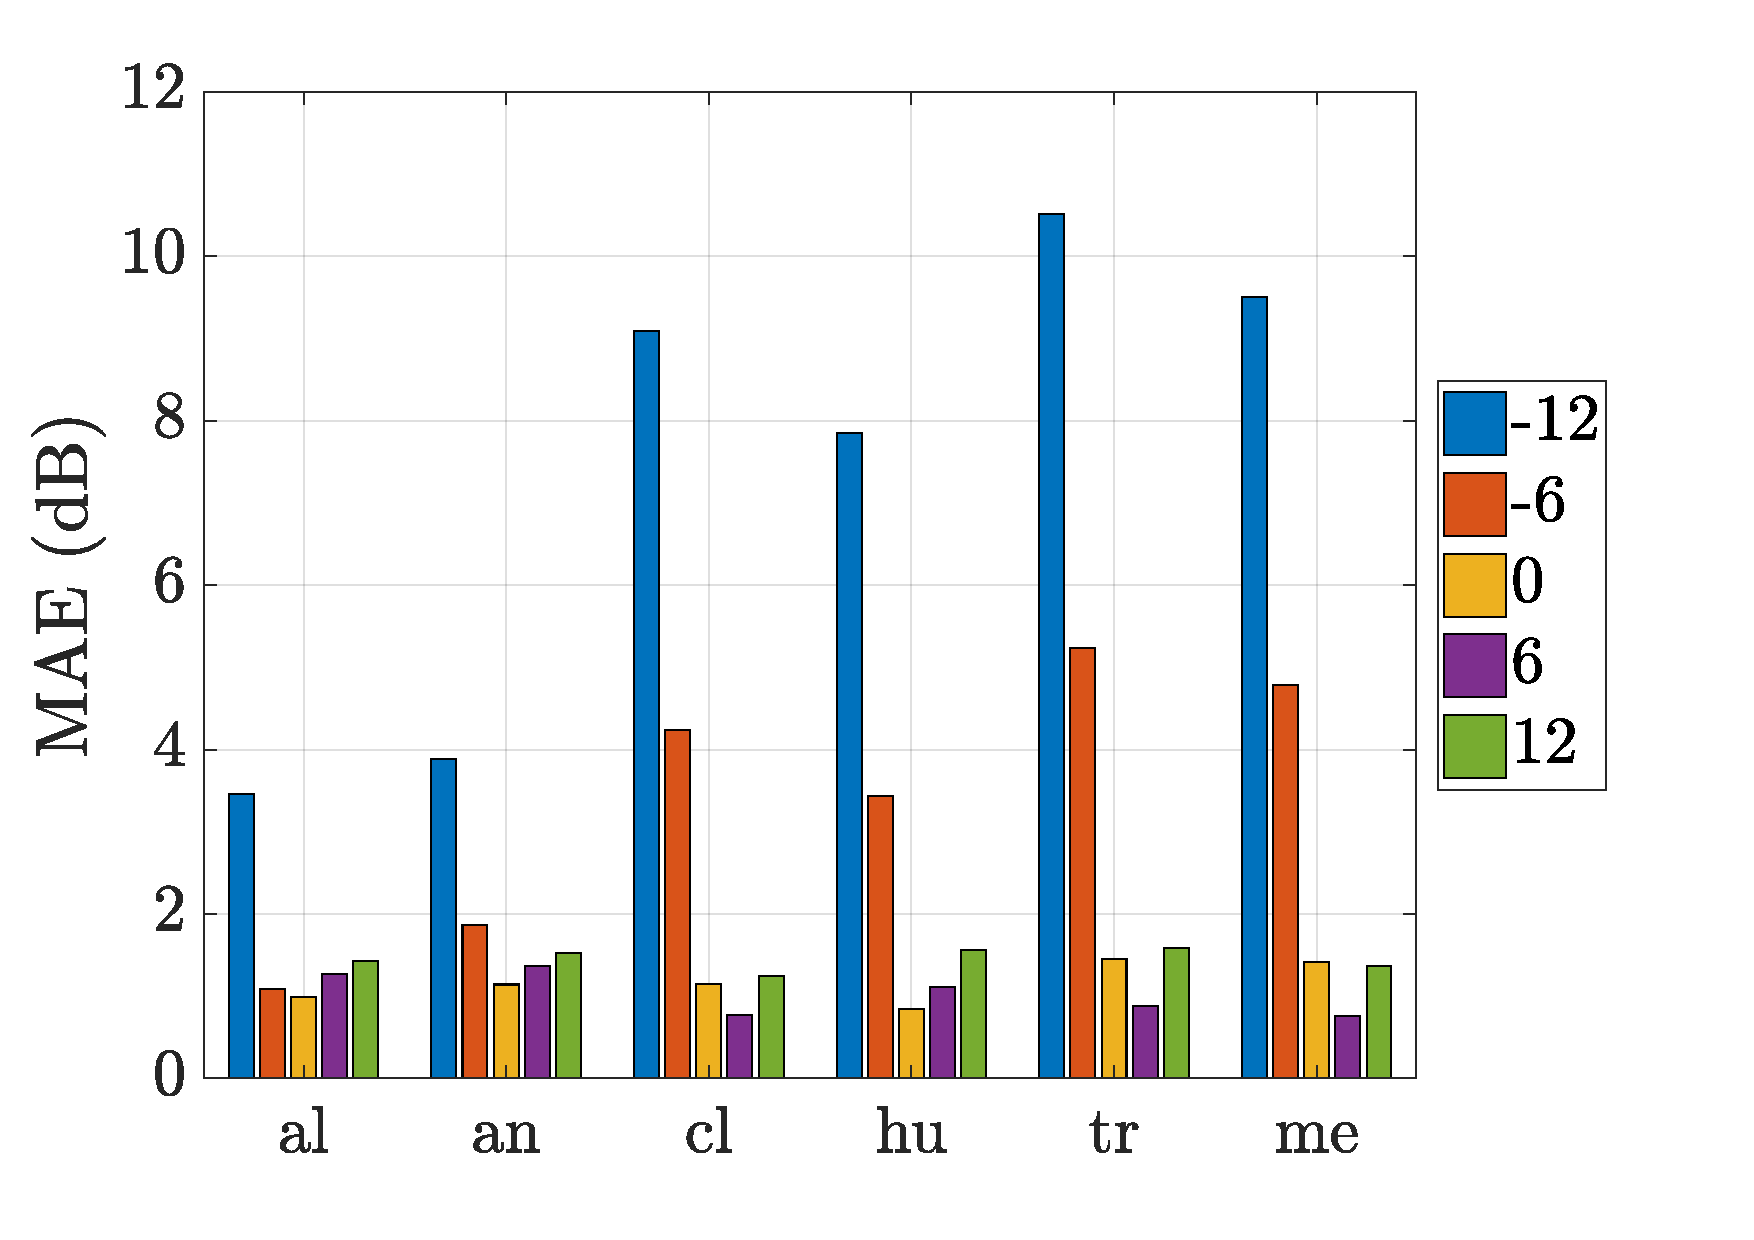
\includegraphics[width=\linewidth]{../image/filter_bar.pdf}
\caption{MAE error for the best cut-off frequency for the filter method according each sub-classes and $TIR$}
\label{tab:filtre_error}
\end{figure}

\begin{figure}[hbtp]
\centering

\caption{MAE error for the best combination parameters for supervised NMF ($\beta = 2$, spectra) according each sub-classes and $TIR$}
\label{tab:Sup_error}
\end{figure}

\begin{figure}[hbtp]
\centering
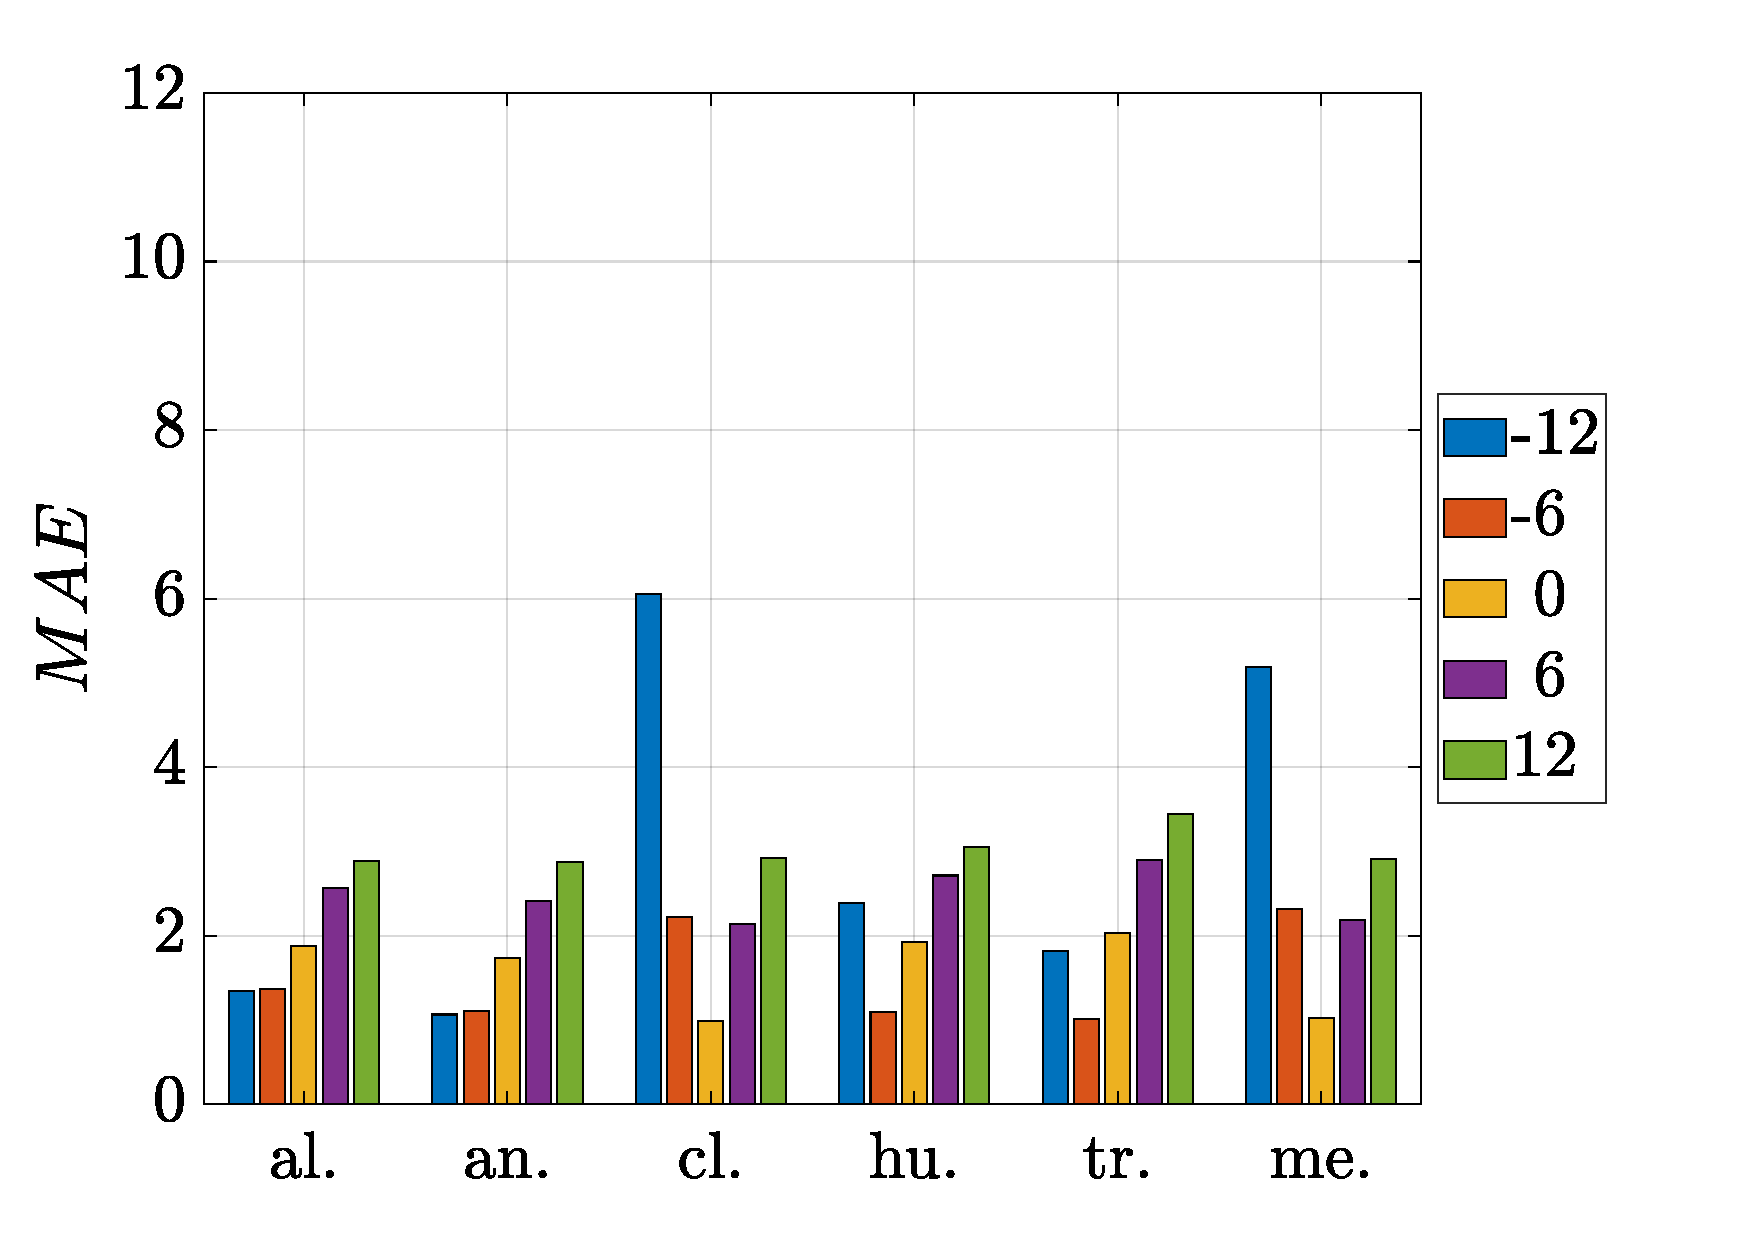
\includegraphics[width=\linewidth]{../image/semi-sup_bar.pdf}
\caption{MAE error for the best combination parameters for semi-supervised NMF ($\beta = 2$, spectra) according each sub-classes and $TIR$}
\label{tab:Semi_error}
\end{figure}

\begin{figure}[hbtp]
\centering
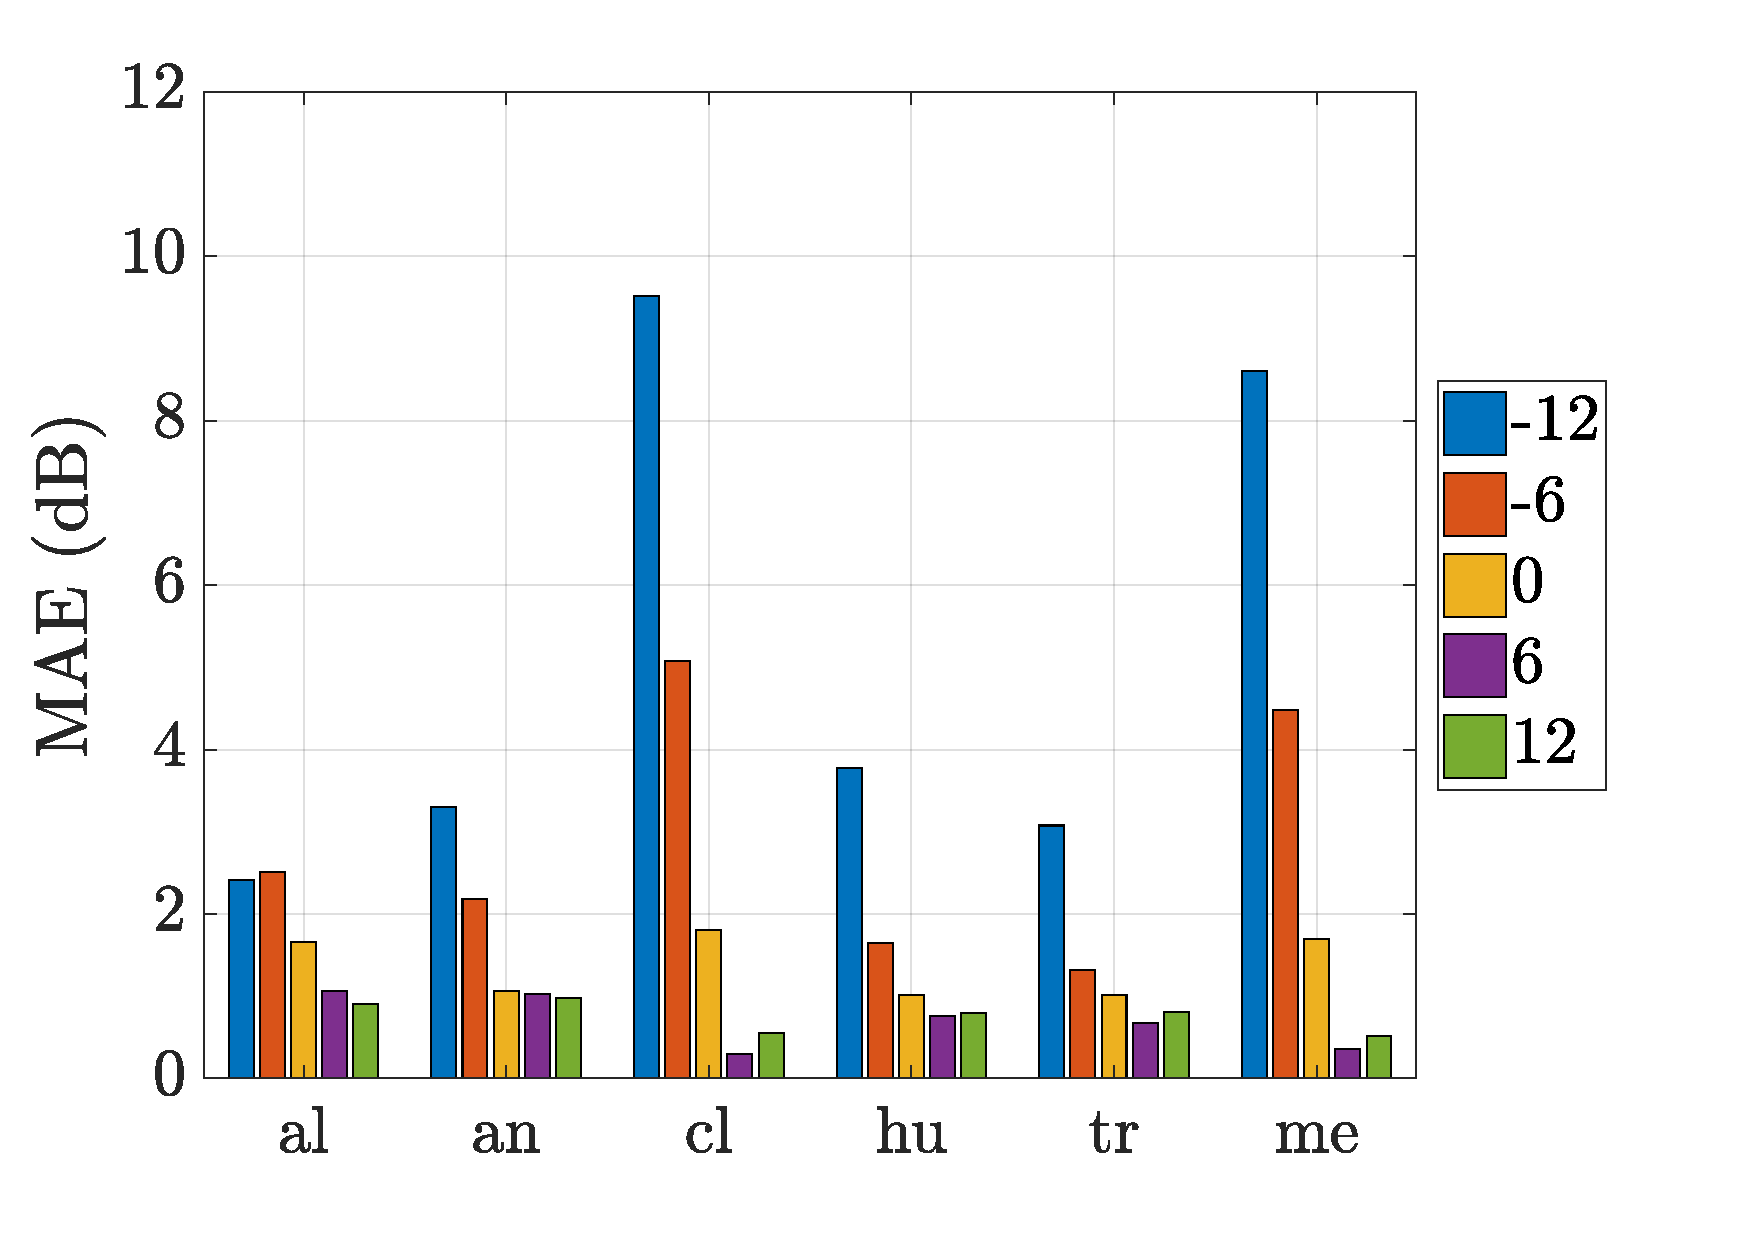
\includegraphics[width=\linewidth]{../image/THC_bar.pdf}
\caption{MAE error for the best combination of parameters for THC NMF ($\beta = 2$, third octave) according each sub-classes and $TIR$}
\label{tab:THC_error}
\end{figure}

The first approach consider is the frequency low-pass filter. With $f_c = 20 kHz$, the error is naturally higher for low $TIR$ (-12,-6) as the traffic is less present. In the opposite, for high $TIR$ (6 and 12), as the traffic become preponderant, the traffic  sound level estimation is better as this method conserve all the traffic energy. A second cut-off frequency, $f_c = 500 Hz$, allow to have a balance as it put aside the high frequencies and to keep low frequencies. It results that for low $TIR$ with high frequencies class sound (\textit{alert}, \textit{animals}), the errors can be low but are high as soon as sound classes are composed of low frequencies (\textit{climate}, \textit{humans}, \textit{transport} and \textit{mechanics}). 



Semi-supervised NMF is efficient particularly for low $TIR$ as the mobile part, $W_r$, allows to take into account the other predominant sound sources while supervised NMF is constrained to use traffic elements to reduce the distance/divergence between $\mathbf{V}$ and $\mathbf{WH}$. Nevertheless, these degrees of freedom are restrictive for high $TIR$. Indeed, semi-supervised NMF is free to include traffic components in $W_r$. The traffic sound level estimation is then less right. In the opposite, for $TIR = [6 , 12]$, supervised NMF has to use the traffic element present in $W$. In this case, the performances are then better. 

Finally, THC NMF with a threshold fixed at $t = 0.54$ is the one where for low and high $TIR$, the performance are lower than the baseline's. The dictionary update allows to the method to adapt to the different $TIR$ and to only keep the closest elements of the \textit{traffic} component \ref{fig:dist_-12_12}.

\begin{figure}
    \centering
    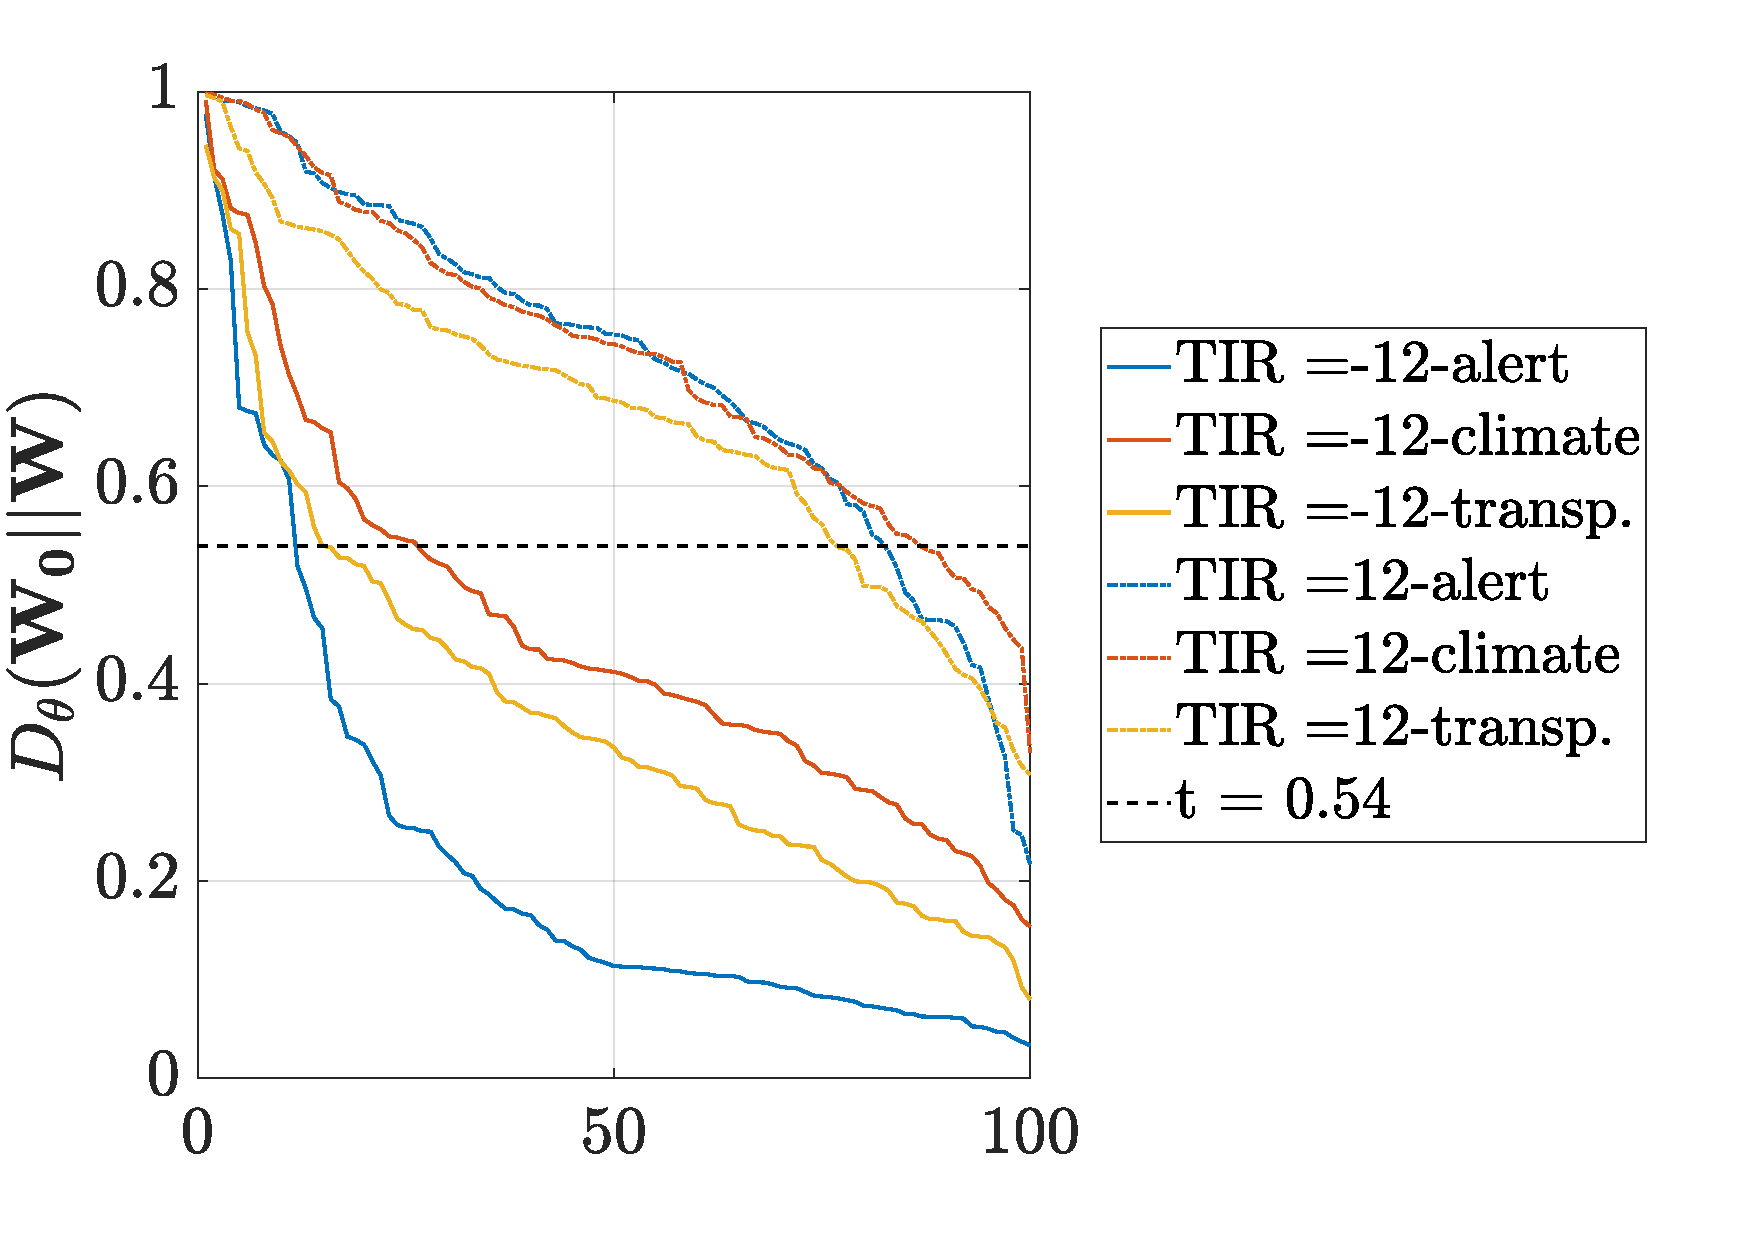
\includegraphics[width=\linewidth]{../image/dist_-12_12.pdf}    
    \caption{Example of the similarity $\cos \theta$ for an sound mixture of the \textit{alert} sub-class for two $TIR$ and with the threshold $t$: $TIR = -12$ (a) and $TIR = 12$ (b)}
    \label{fig:dist_-12_12}
\end{figure}



%\subsection{Frequency low-pass filter results}
%In a first time, the frequency low-pass filter estimator is performed on all the scene. The table \ref{tab:results_filter} summarized the mean error on the totality of the 750 scenes to find the most efficient cut-off frequency. \\
%
%\begin{table}[h]
%\centering
%\begin{tabular}{llll}
%$f_c$ (Hz) & $MAE$ (dB) & $nRMSE$  \\ \hline
% 500 & \textbf{\textcolor{red}{5.66 $\pm$6.59}} & \textbf{\textcolor{red}{1.48 $\pm$1.10}} \\
% 1000 & \textbf{6.31 $\pm$7.64} & \textbf{1.52 $\pm$1.34} \\
% 2000 & \textbf{6.65 $\pm$8.24} & \textbf{1.57 $\pm$1.54} \\
% 5000 & \textbf{7.42 $\pm$8.90} & 1.82 $\pm$1.65 \\
%10000 & \textbf{7.55 $\pm$9.00} & 1.89 $\pm$1.70 \\
%20000 & \textbf{7.59 $\pm$9.02} & 1.89 $\pm$1.72 \\
%\end{tabular}
%\caption{RMSE error for the low pass filter averaged on all the TIR and sub-classes}
%\label{tab:results_filter}
%\end{table}
%
%According the table \ref{tab:results_filter}, the cut-off frequency at 500 Hz is the most efficient on all the TIR and all the sub-classes. The corresponding errors according to the sub-classes and the TIR are summarized in the figure \ref{fig:filterAmbiance}.\\
%
%\begin{figure}[t]
%\centering
%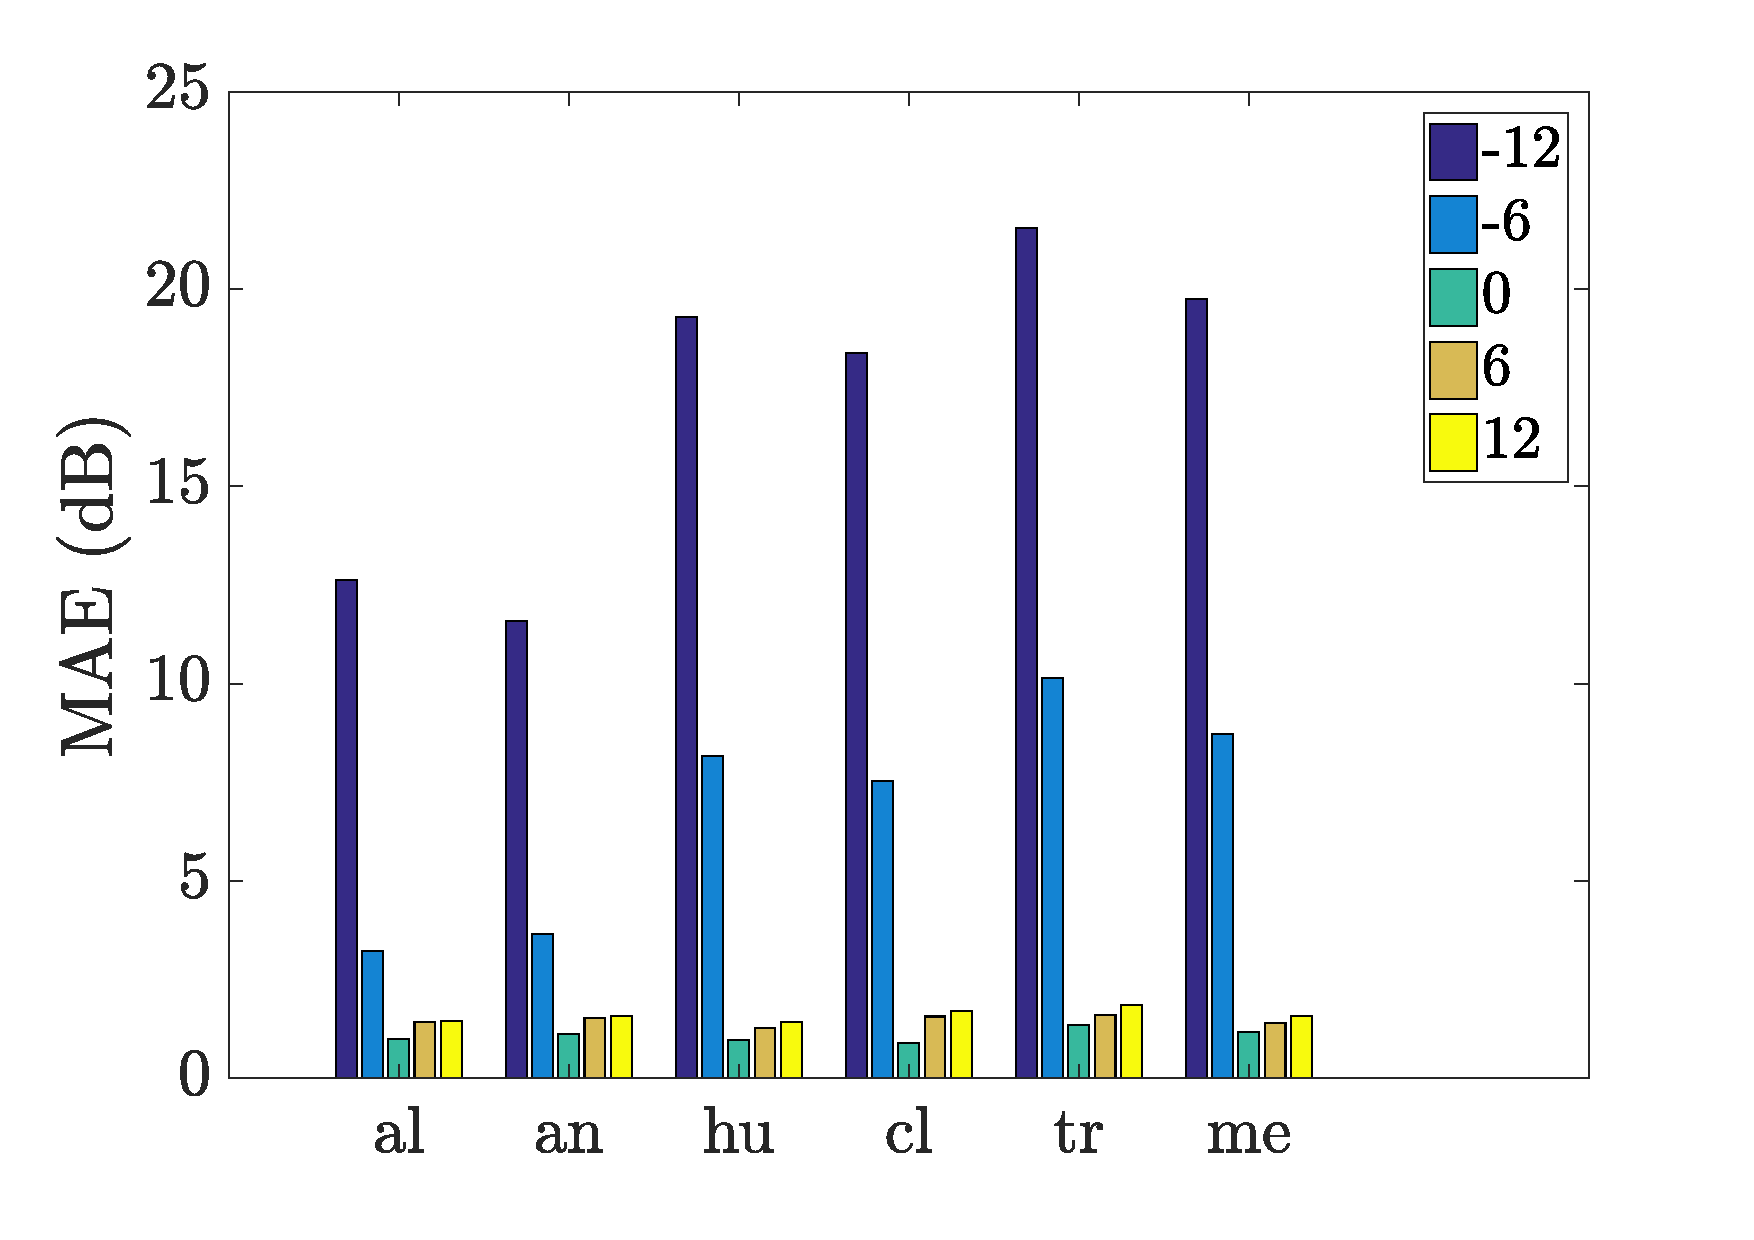
\includegraphics[width=\linewidth]{../image/AmbianceFilter.pdf}
%\caption{Bar plot for the filter according to the sub-classes and the TIR at $f_c$ = 500 Hz cut-off frequency}
%\label{fig:filterAmbiance}
%\end{figure}
%
%The error for all the sub-corpus is important for the low TIR (-12 and -6) due to the confusion between the \textit{interfering} class and the \textit{traffic} class. The error is less for the \textit{alert} and \textit{humans} sub-corpus as it is composed of higher frequencies while, for other sub-classes, the error are far more important. For the higher \textit{TIR}, the traffic is more present and become dominating on the \textit{interfering} class. The lower error, here, is due to the suppression of the traffic energy by the filter. Finally, the error for $f_c = 20$ kHz is equivalent to the one produced when the \textit{traffic} and the \textit{interfering} classes are take into account together without distinction.
%
%\subsection{Supervised NMF results}
%
%As it is not possible to summarize all the parameter combinations, just the best results according to the domain and $\beta$ at the $\nth{400}$ iteration are presented in table \ref{tab:results_supervised}. The bar plot in figure \ref{fig:nmfSupervisedAmbiance} displays the $MAE$ error for the best combination.\\
%
%\begin{table*}[t]
%\centering
%\begin{tabular}{lllllcc}
%$K$ & \shortstack{temporal\\window (ms)} & domain & $f_c$ (Hz) & $\beta$ & $MAE$ (dB) & $nRMSE$ \\
%\hline
% 25 & 500 & spectra &  2000 & 1 & \textbf{6.18 $\pm$7.49} & \textbf{1.48 $\pm$1.20} \\
% 25 & 500 & spectra &   500 & 2 & \textbf{\textcolor{red}{5.32 $\pm$6.28}} & \textbf{1.40 $\pm$0.93} \\
% 25 & 0 & third octave & 20000 & 1 & \textbf{6.82 $\pm$8.16} & 1.60 $\pm$1.34\\
% 25 & 500 & third octave & 20000 & 2 & \textbf{6.26 $\pm$7.69} & \textbf{\textcolor{red}{1.36 $\pm$1.19}} \\
%\end{tabular}
%\caption{RMSE error for supervised NMF averaged on all the TIR and sub-classes}
%\label{tab:results_supervised}
%\end{table*}
%
%\begin{figure}[h]
%\centering
%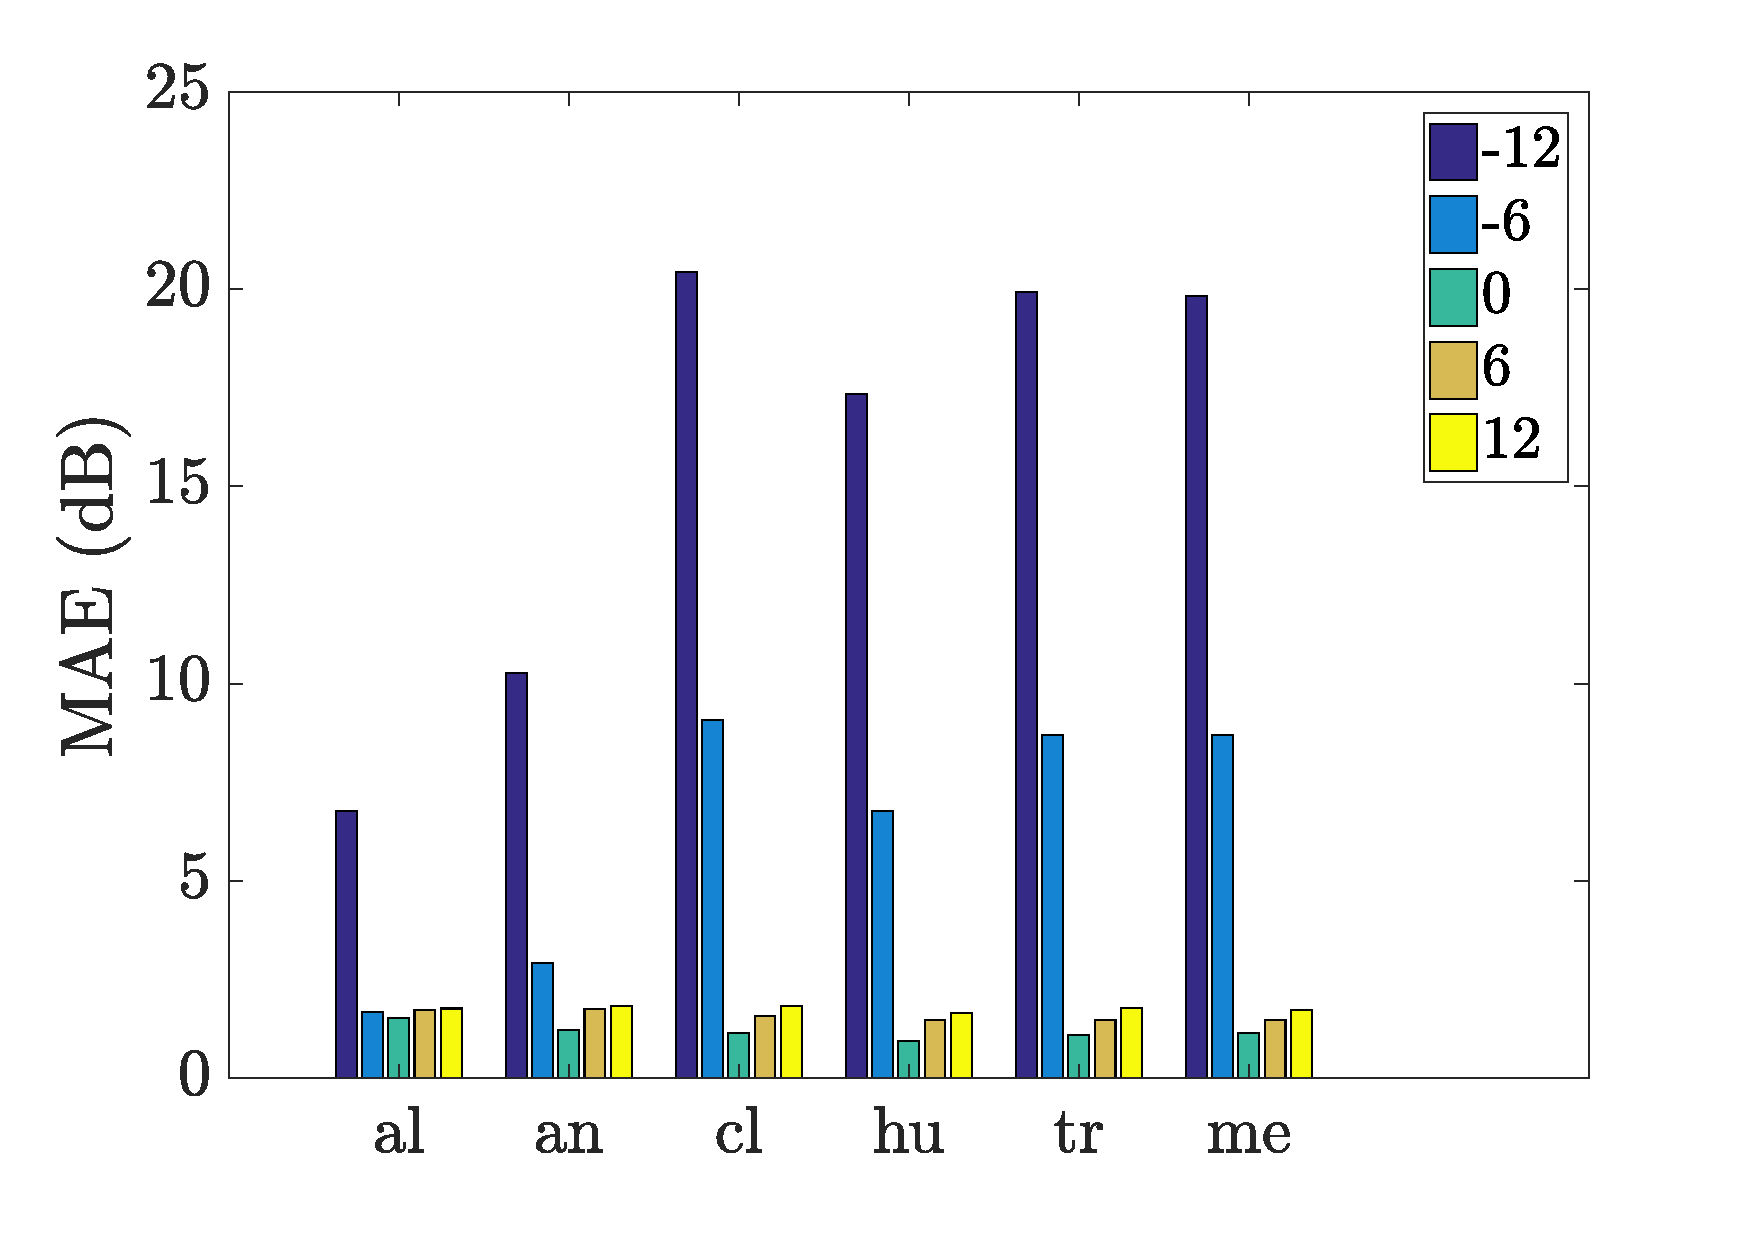
\includegraphics[width=\linewidth]{../image/AmbianceNmfSupervised.pdf}
%\caption{bar plot for the best parameter combination of the supervised NMF ($K = 25$, temporal window = 0.5 s, domain = spectra, $\beta$ = 2, $f_c$ = 500 Hz )}
%\label{fig:nmfSupervisedAmbiance}
%\end{figure}
%
%\begin{table}[h]
%\centering
%\begin{tabular}{ccc}
%    & \multicolumn{2}{c}{$MAE$ (dB)} \\ \hline
%TIR & filtre & supervised NMF \\ \hline
% -12 & 17.20 $\pm$ 4.09 & 15.76 $\pm$ 5.82 \\
% -6 &  6.91 $\pm$ 2.82 & 6.32 $\pm$ 3.24\\
% 0 & 1.09 $\pm$ 0.16 & 1.18 $\pm$ 0.19\\
%  6 &  1.47 $\pm$ 0.12 & 1.59 $\pm$ 0.13\\
% 12 &  1.60 $\pm$ 0.16 & 1.77 $\pm$ 0.07
%\end{tabular}
%\caption{Comparison of the $MAE$ error for the filter at 500 Hz and the best combinaison of the supervised NMF}
%\label{tab:resultsComparison}
%\end{table}
%
%
%The best combination for supervised NMF is the one with described in the \textit{spectra} domain and for the euclidean distance with $K = 25$, a temporal window of 500 ms and $f_c = 500$ Hz. The errors produced by NMF, on the totality of the scenes, is smaller than the filter approach for all the metrics. For the higher \textit{TIR}, both methods have similar performances (table \ref{tab:resultsComparison}). For the lower \textit{TIR}, TIR, supervised NMF reduces significantly the error. By distinguishing each class, it is lower for the \textit{alert} and \textit{animals} than the rest sub-classes. \\
%
%This difference can be illustrate through the evolution of the cost function (figures \ref{fig:costSup12}) and of the $MAE$ error (figure \ref{fig:EarlyStop12}) for 3 sub-classes (\textit{alert}, \textit{climate} and \textit{transportation}), for 2 \textit{TIR} (-6 and 6) until the $\nth {100}$ iterations.\\
%
%\begin{figure}
%    \centering
%    \subfigure[]{\label{fig:EarlyStop1}
%    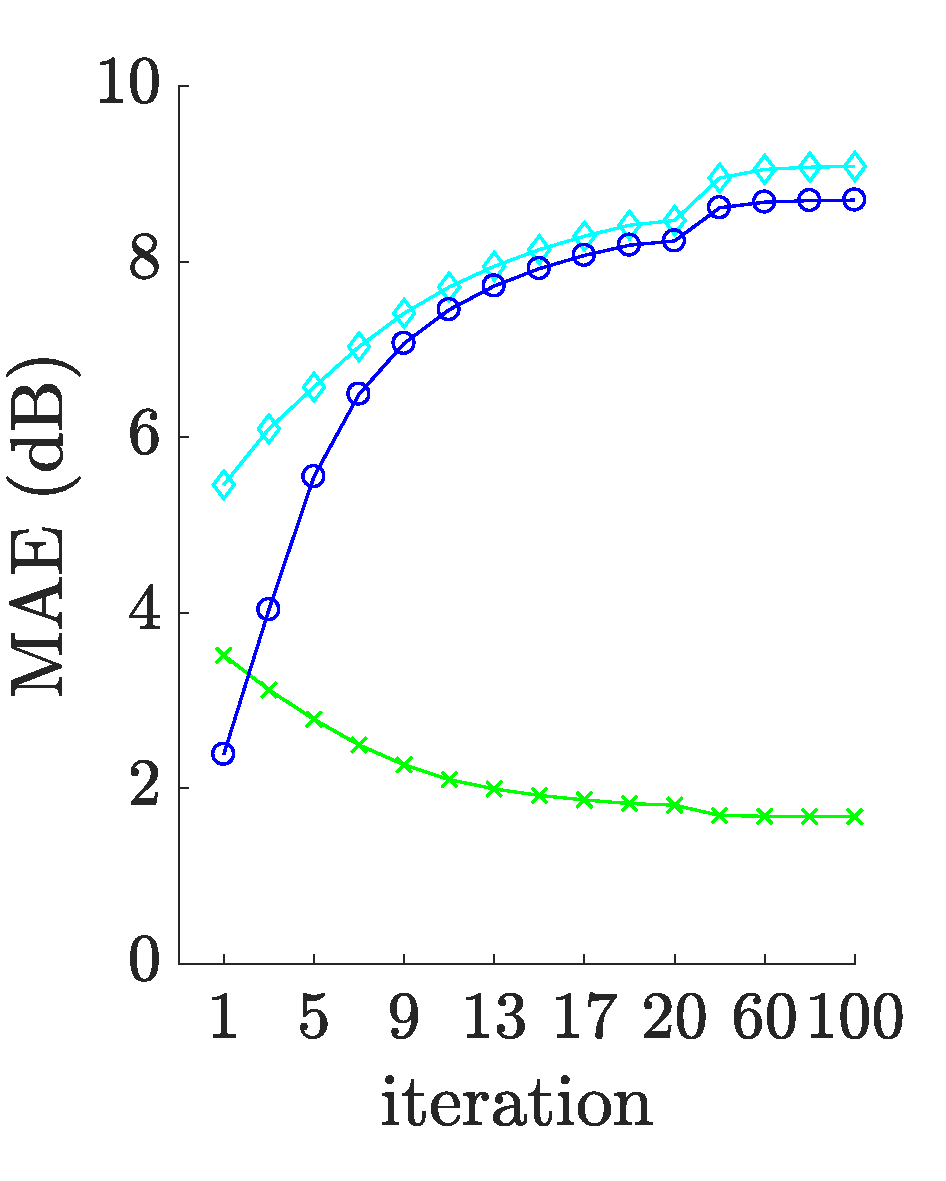
\includegraphics[width=0.45\linewidth]{../image/AmbianceNmfSupervised_EarlyStop_TIR-6.pdf}}
%    \subfigure[]{\label{fig:EarlyStop2} 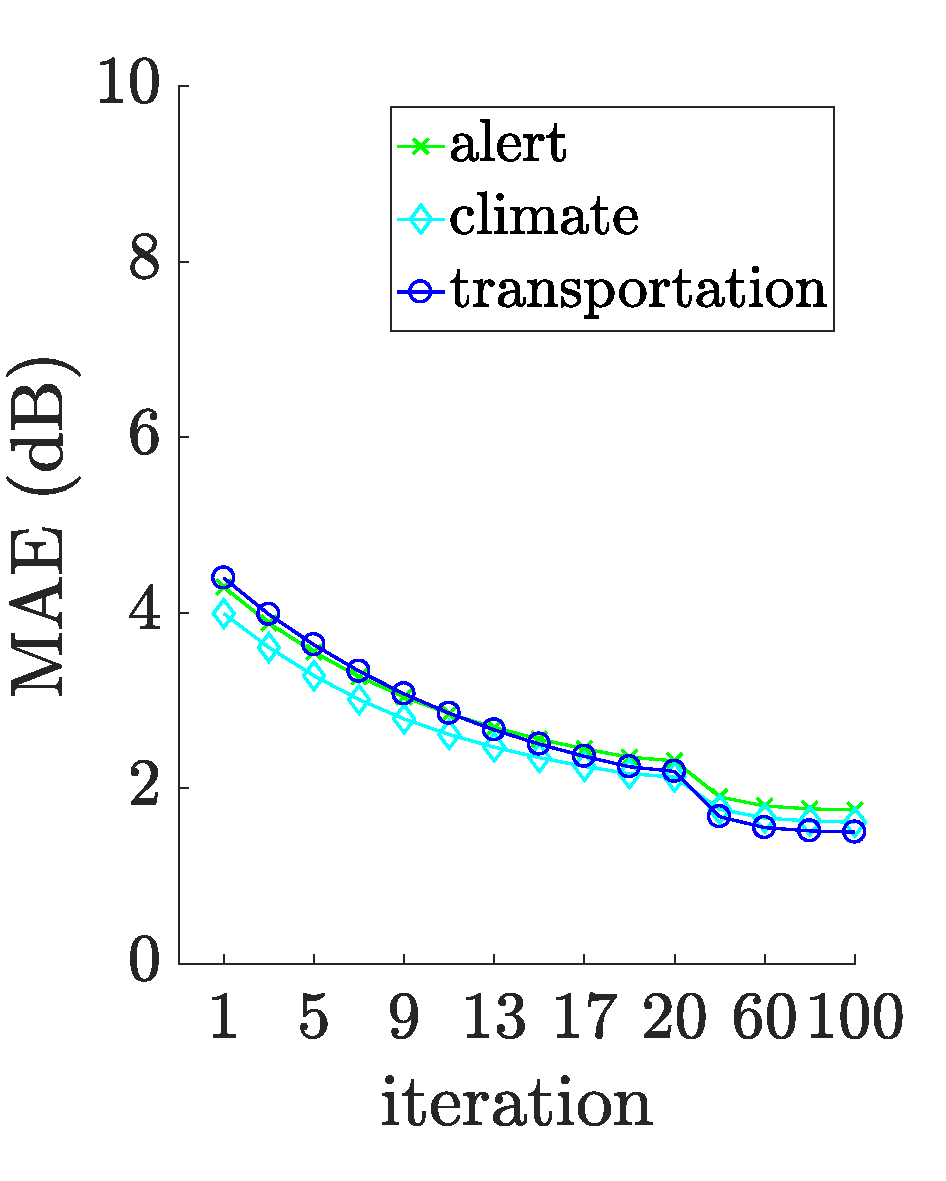
\includegraphics[width=0.45\linewidth]{../image/AmbianceNmfSupervised_EarlyStop_TIR6.pdf}}
%    \caption{Evolution of the $MAE$ for 3 sub-classes for TIR = -6 (fig.  \ref{fig:EarlyStop1}) and TIR = 6 (fig. \ref{fig:EarlyStop2})}
%    \label{fig:EarlyStop12}
%\end{figure}
%
%\begin{figure}
%    \centering
%    \subfigure[]{\label{fig:costSup1}
%    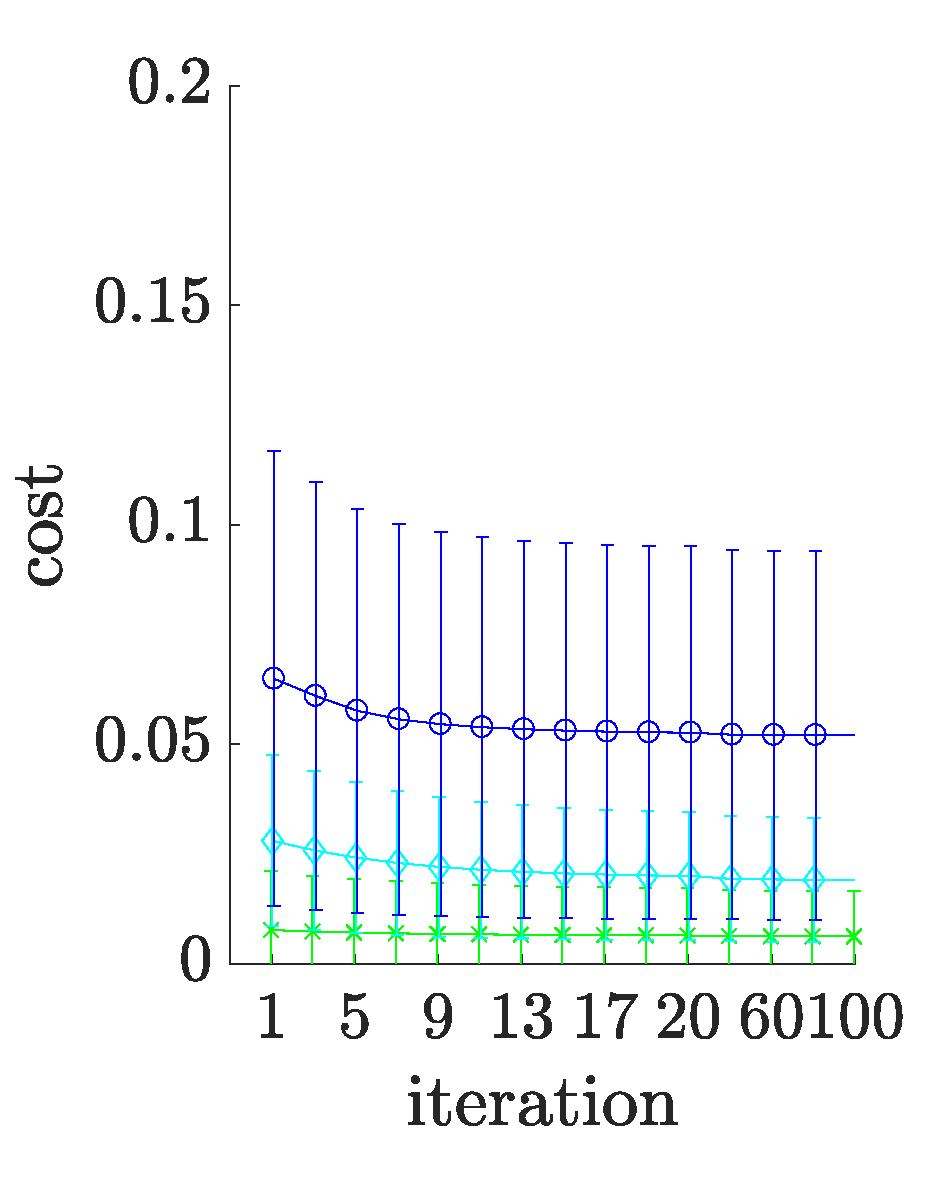
\includegraphics[width=0.45\linewidth]{../image/AmbianceNmfSupervised_EarlyStop_TIR-6Cost.pdf}}
%    \subfigure[]{\label{fig:costSup2} 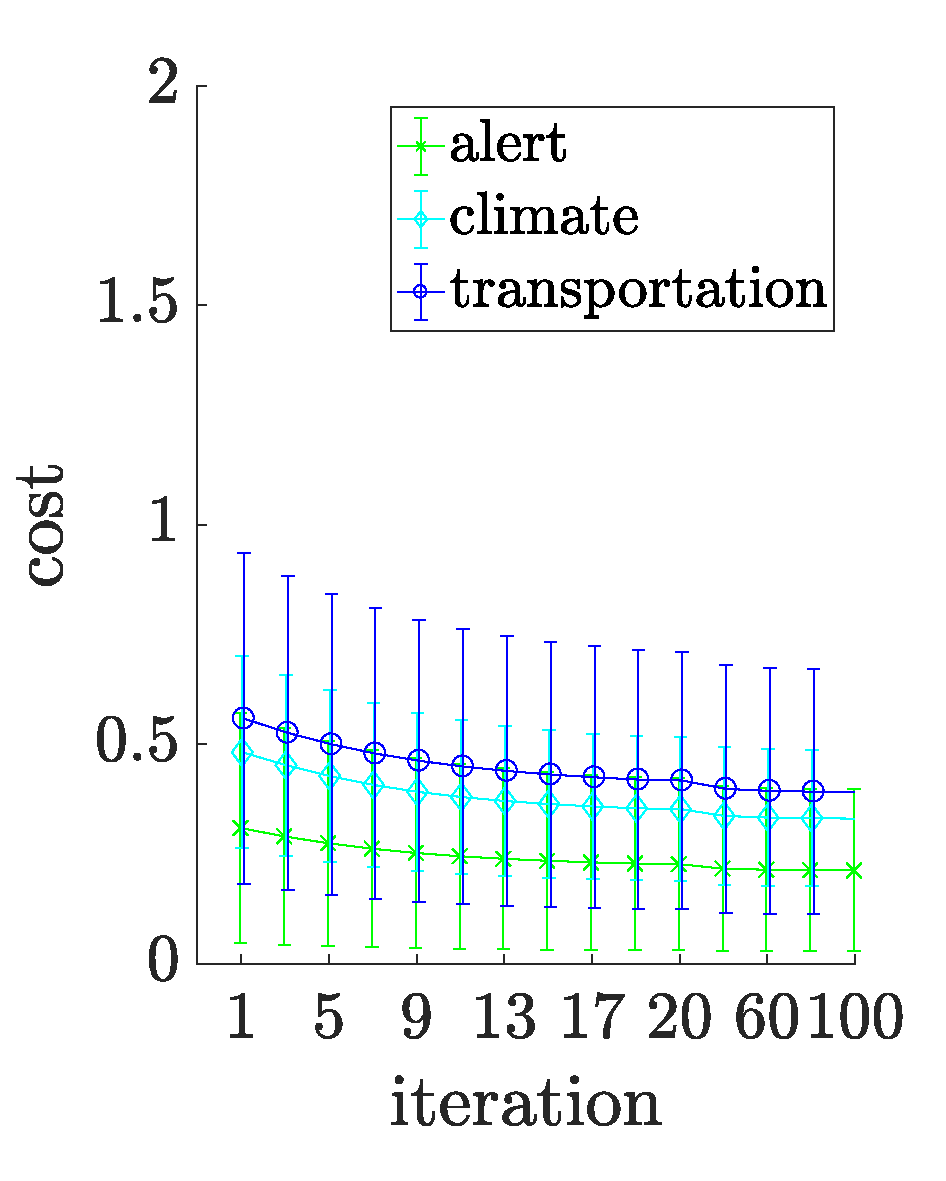
\includegraphics[width=0.45\linewidth]{../image/AmbianceNmfSupervised_EarlyStop_TIR6Cost.pdf}}
%    \caption{Evolution of the $MAE$ for 3 sub-classes for TIR = -6 (fig.  \ref{fig:costSup1}) and TIR = 6 (fig. \ref{fig:costSup2})}
%    \label{fig:costSup12}
%\end{figure}
%
%For the TIR = 6, the cost function and the $MAE$ error are decreasing, meaning the global mixture and the traffic signal are well synthesized. Here as the $\mathbf{W}$ is only composed of traffic elements and the sound scenes are composed of a predominant traffic, the reconstruction of the signal is easier. In opposite, for the case where \textit{TIR} = -6, for the \textit{alert} signal, the cost function and the $MAE$ error are decreasing too. But for the \textit{climate} and \textit{transportation} sub-classes, the $MAE$ error is increasing. Even if the cost function decreases, the quality of the traffic signal rebuilt is not improved. This difference can be explained by the type of sound present in these different sub-classes: for \textit{alert} and \textit{animals}, it includes harmonic sounds which belong in the frequency range $\left[2000-5000\right]$ Hz while the other sub-classes include lower frequency sounds.  As $\mathbf{W}$ is composed of traffic spectrum, located in low frequencies too, it is more difficult to recompose correctly the traffic signal when the \textit{interfering} sound is predominant and composed of low frequencies too. As NMF minimized the cost function (equation \ref{eq:min-D-WH}), \textit{traffic} spectrum then are used to synthesized the global mixture at the expense of the traffic signal.
%
%\subsection{Semi-supervised NMF results}
%
%The errors produced for the semi-supervised approach is summarized in table \ref{tab:results_semi_supervised} according to $\beta$ and the frequency domain (spectral or third octave).\\
%
%\begin{table*}
%\centering
%\begin{tabular}{cclllccc}
%$K$ & \shortstack{temporal\\window (ms)} & $f_c$ (Hz) & domain & $\beta$ & $MAE$ (dB) & $nRMSE$ \\
%\hline
% 50 & 0 & spectra &  1000 & 1 & \textbf{4.50 $\pm$3.05} & 1.45 $\pm$0.76 \\
%100 & 0 & spectra & 20000 & 2 & \textbf{4.05 $\pm$3.43} & \textbf{\textcolor{red}{1.16 $\pm$0.53}} \\
% 25 & 0 & third octave & 20000 & 1 & \textbf{\textcolor{red}{3.96 $\pm$2.18}} & 1.34 $\pm$0.72 \\
% 25 & 0 & third octave & 20000 & 2 & \textbf{4.29 $\pm$3.58} & \textbf{1.21 $\pm$0.61}
%\end{tabular}
%\caption{RMSE error for semi-supervised NMF averaged on all the TIR and sub-classes}
%\label{tab:results_semi_supervised}
%\end{table*}
%
%The best combination is got in the third octave domain with $\beta = 1$, $f_c$ = 20 kHz, $K$ = 25 and a temporal window null. The error, compared to the supervised approach, is lower. Furthermore, the standard deviation is lower too meaning that the semi-supervised approach offer a much more stable error than the previous method. The figure \ref{fig:nmfSemiSupervisedAmbiance} displayed the error for the best scenario averaged on all the sub-classes and the \textit{TIR}. The table \ref{tab:comparisonFilterSemiSupervised} summarizes the error expanded to the \textit{TIR}.
%
%\begin{figure}[hbtp]
%\centering
%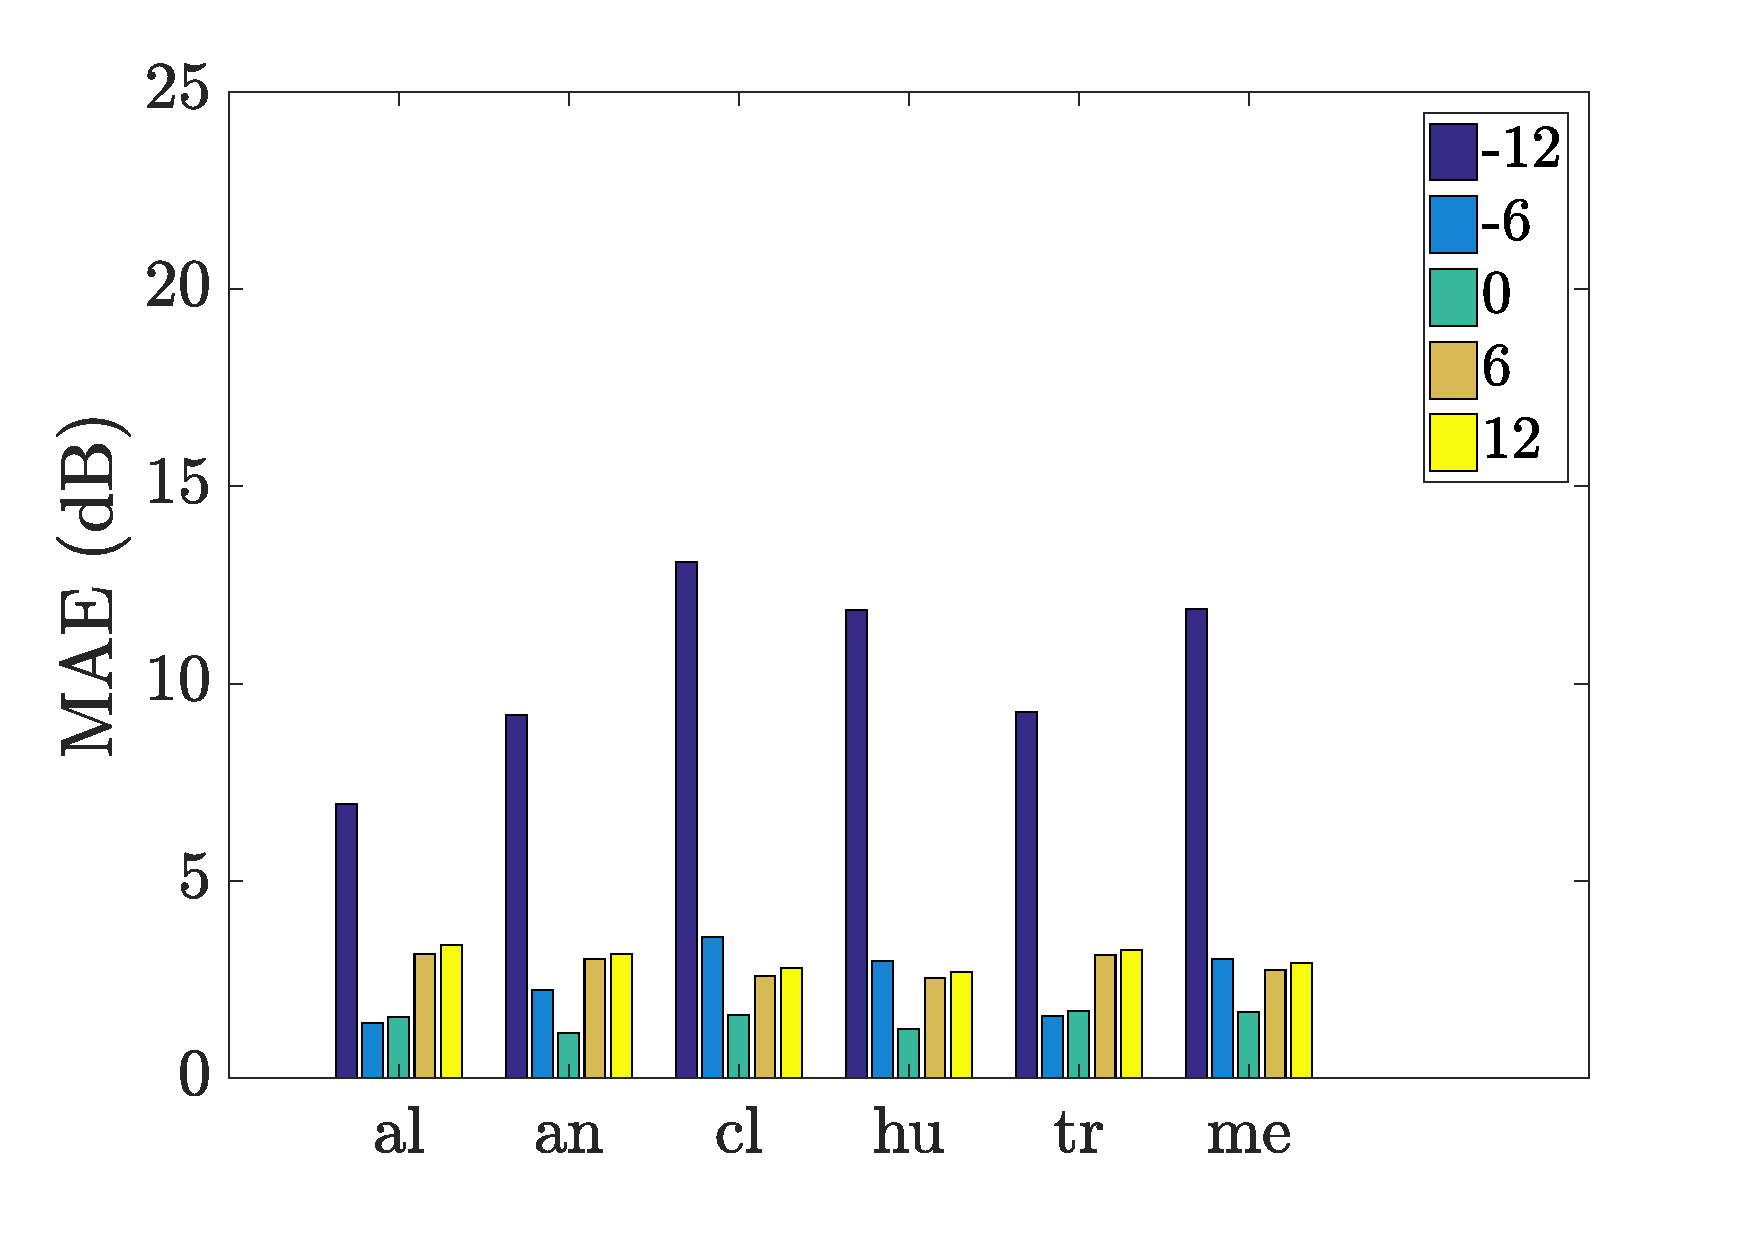
\includegraphics[width=\linewidth]{../image/AmbianceNmfSemiSupervised.pdf}
%\caption{bar plot for the best parameter combination of the supervised NMF ($K = 25$, temporal window = 0.5 s, domain = spectra, $\beta$ = 2, $f_c$ = 20 kHz)}
%\label{fig:nmfSemiSupervisedAmbiance}
%\end{figure}
%
%\begin{table}
%\centering
%\begin{tabular}{cccc}
%    & \multicolumn{2}{c}{$MAE$ (dB)} \\ \hline
%TIR & filter & semi-Supervised NMF \\ \hline
% -12 & 17.20 $\pm$4.09 &  7.46 $\pm$2.88 \\
% -6 &  6.91 $\pm$2.82 & 2.15 $\pm$0.70\\
% 0 & 1.09 $\pm$0.16 &  2.20 $\pm$0.45\\
% 6 &  1.47 $\pm$0.12 &  3.61 $\pm$0.29\\
% 12 &  1.60 $\pm$0.16 &  4.02 $\pm$0.33\\
%\end{tabular}
%\caption{Comparison of the baseline and semi-supervised NMF with the best combination}
%\label{tab:comparisonFilterSemiSupervised}
%\end{table}
%
%The error for low TIR is much lower than the filter or supervised NMF. The add of the mobile part makes NMF less constraint and therefore allows to adapt NMF to low traffic contents. Figure display the mobile part of the dictionary, $\mathbf{W_r}$ for two particular sub-classes (\textit{alert} and \textit{climate} and for \textit{TIR} = -6.\\
%
%
%\textbf{figure $W_r$ for alert and climate}\\
%
%Nevertheless, the advantage won with the mobile part, generates larger errors in higher \textit{TIR}. Here, NMF uses $\mathbf{W_r}$ in order to minimize the cost function. As the mobile part is not constraint, traffic content is included in it, decreasing the quality of the traffic signal reconstruction. Figure display the 2 basis of $\mathbf{W_r}$. \\
%
%\textbf{figure $W_r$ for alert and climate}\\
%
%These behaviors can be noticed through the $MAE$ evolution in figures \ref{fig:EarlyStopSemi12}: for low TIR the error is decreasing like the cost function (figure \ref{fig:costSemiSup1}) meaning that the synthesis of the traffic signal is good. For the \textit{alert} sub-class, $\mathbf{W_r}$ enables to include the harmonic component which are not present in $\mathbf{W_s}$, the improvement bring by the semi-supervised approach is then remarkable. Whereas, in \textit{climate} sub-class, the \textit{interfering} sound classes are composed of low-frequencies that are present in $\mathbf{W_s}$. This class might be describe with the help of $\mathbf{W_s}$.
%
%For \textit{TIR} = 6, the error is increasing for all sub-classes. As the objective function is to minimize the distance between the spectrogram $\mathbf{V}$ and $\mathbf{WH}$, the semi-supervised approach is free to include traffic component in $\mathbf{W_r}$ to do it. This degree of freedom deteriorates the reconstruction of the traffic signal. \\
%
%\begin{figure}
%    \centering
%    \subfigure[]{\label{fig:EarlyStopSemi1}
%    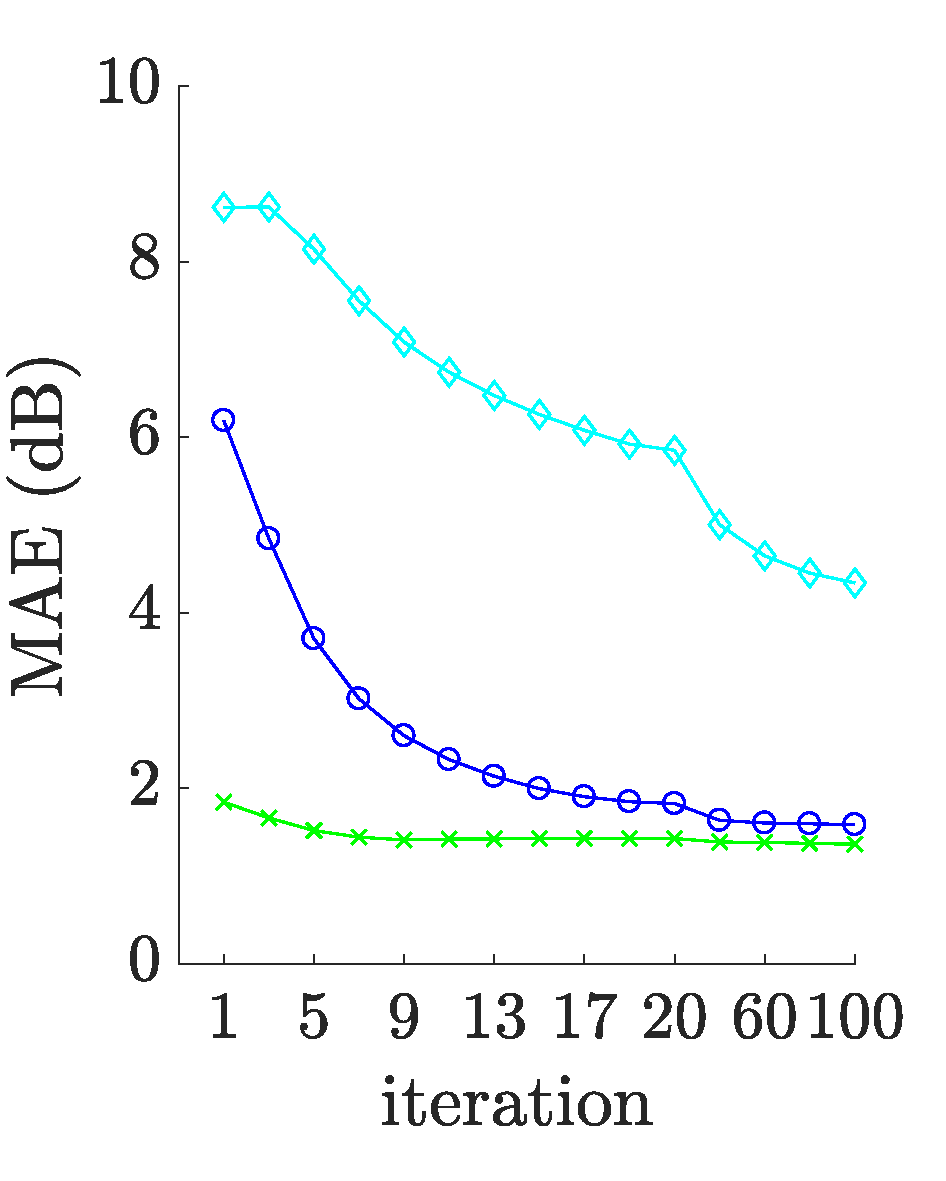
\includegraphics[width=0.45\linewidth]{../image/AmbianceNmfSemiSupervised_EarlyStop_TIR-6.pdf}}
%    \subfigure[]{\label{fig:EarlyStopSemi2} 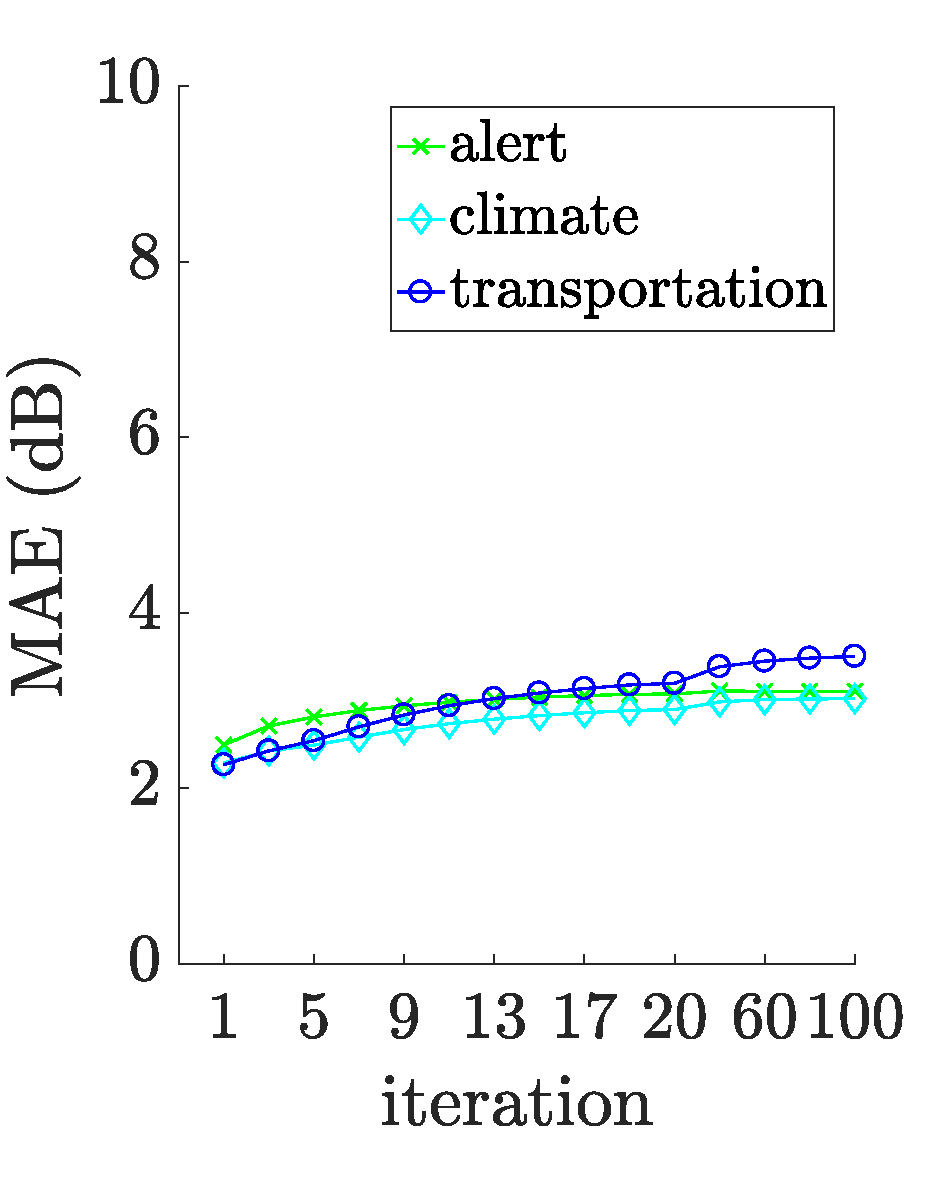
\includegraphics[width=0.45\linewidth]{../image/AmbianceNmfSemiSupervised_EarlyStop_TIR6.pdf}}
%    \caption{Evolution of the $MAE$ for 3 sub-classes for TIR = -6 (fig.  \ref{fig:EarlyStopSemi1}) and TIR = 6 (fig. \ref{fig:EarlyStopSemi2})}
%    \label{fig:EarlyStopSemi12}
%\end{figure}
%
%\begin{figure}
%    \centering
%    \subfigure[]{\label{fig:costSemiSup1}
%    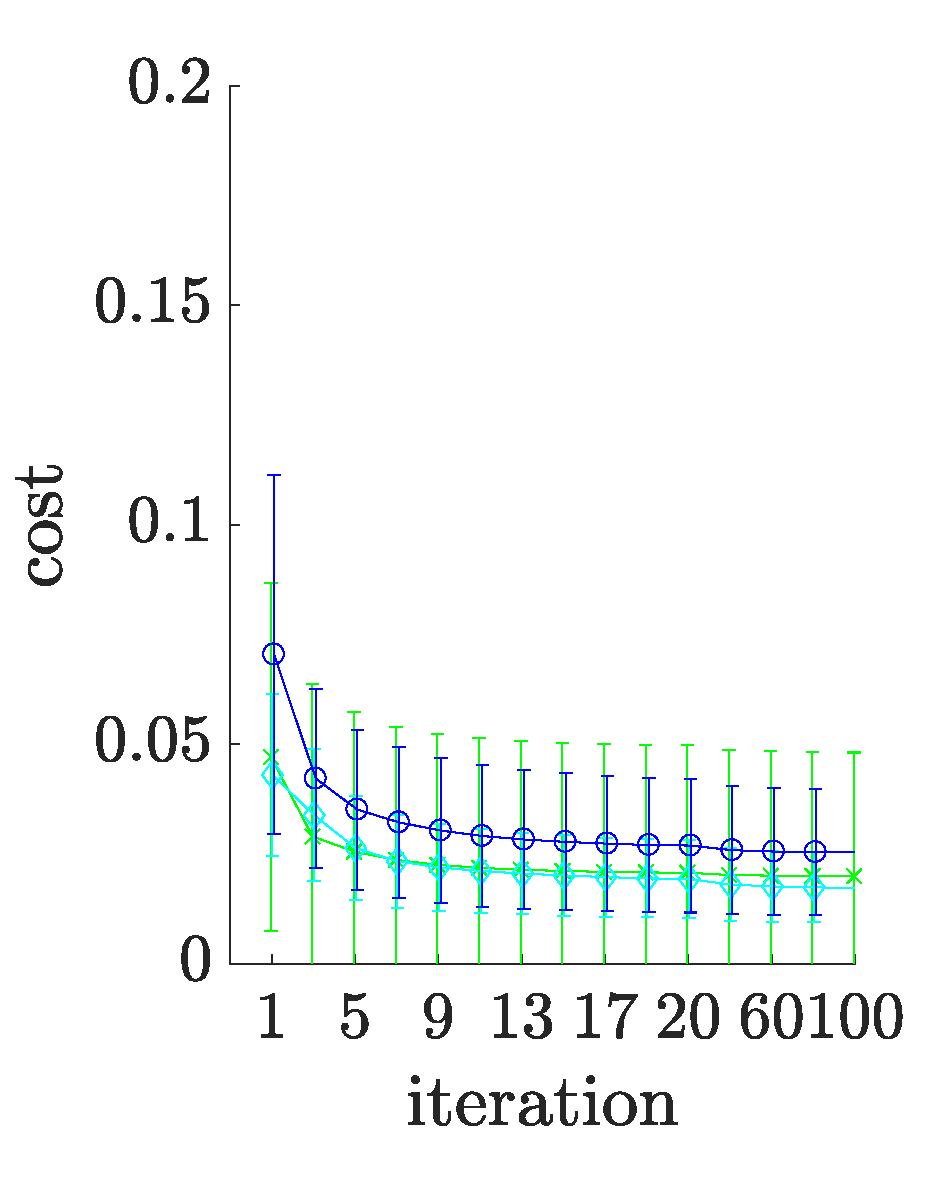
\includegraphics[width=0.45\linewidth]{../image/AmbianceNmfSemiSupervised_EarlyStop_TIR-6Cost.pdf}}
%    \subfigure[]{\label{fig:costSemiSup2} 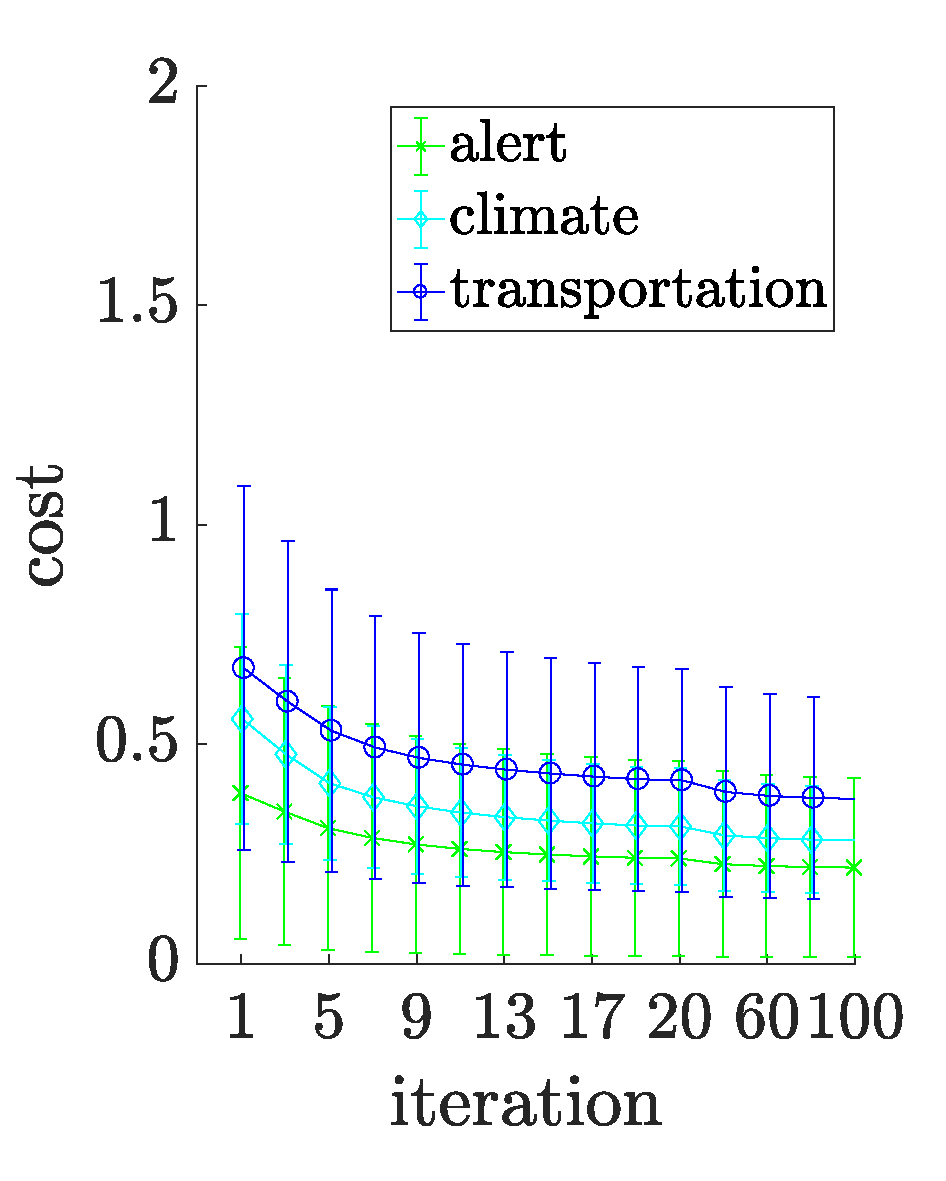
\includegraphics[width=0.45\linewidth]{../image/AmbianceNmfSemiSupervised_EarlyStop_TIR6Cost.pdf}}
%    \caption{Evolution of the $MAE$ for 3 sub-classes for TIR = -6 (fig.  \ref{fig:costSemiSup1}) and TIR = 6 (fig. \ref{fig:costSemiSup2})}
%    \label{fig:costSemiSup12}
%\end{figure}
%
%\textbf{miss the evolution of the Lp for the 25 scenes, estimate and exact + 2/3 scenes to see the evolution during the 30 seconds of the scenes ?}

\section{Conclusion}
\footnotesize
\bibliographystyle{unsrt}
\bibliography{bibliographie_applied}

\end{document}
